% !TEX program = xelatex
% Standalone source. Compile twice with XeLaTeX or Tectonic; Fandol fonts are part of TeX Live.
\documentclass[UTF8,11pt,a4paper,fontset=fandol]{ctexart}
% 主文件用 \documentclass[UTF8,11pt,a4paper,fontset=fandol]{ctexart}。
% 通用视觉底座。教学顺序、助教台词、署名与题目由主文件决定。
\usepackage[left=19mm,right=19mm,top=18mm,bottom=18mm,headheight=15pt,headsep=6mm,footskip=9mm]{geometry}
\usepackage{amsmath,amssymb,graphicx,xcolor,fancyhdr,tabularx,booktabs,tikz}
\usetikzlibrary{calc,arrows.meta,angles,quotes,intersections,positioning}
\IfFontExistsTF{Kaiti SC}{\setCJKfamilyfont{zhkai}[BoldFont={Kaiti SC Bold}]{Kaiti SC}}{}

\definecolor{BrickRed}{HTML}{A74636}
\definecolor{RoyalBlue}{HTML}{285C89}
\definecolor{handoutink}{HTML}{242B33}
\definecolor{handoutmuted}{HTML}{59636C}
\setlength{\parindent}{0pt}
\setlength{\parskip}{5pt}
\linespread{1.08}
\setlength{\emergencystretch}{3em}

\newcommand{\HandoutHeader}[3][]{%
  \pagestyle{fancy}\fancyhf{}
  \fancyhead[L]{\small #2}\fancyhead[R]{\small #3}
  \fancyfoot[L]{\scriptsize\fangsong #1}\fancyfoot[R]{\small\thepage}
  \renewcommand{\headrulewidth}{.3pt}}
\newcommand{\HandoutLesson}[2]{%
  \par{\small\heiti\color{BrickRed}#1}\par\vspace{3pt}
  {\fontsize{21}{27}\selectfont\heiti\bfseries #2}\par
  \textcolor{BrickRed}{\rule{\linewidth}{.7pt}}\par}
\newcommand{\HandoutBlock}[1]{\par\vspace{4pt}{\large\heiti\bfseries #1}\par}
\newcommand{\HandoutNote}[1]{\par{\fangsong\fontsize{10.3}{15}\selectfont\color{handoutmuted}#1\par}}
\newcommand{\HandoutBox}[1]{%
  \par\noindent\begingroup\setlength{\fboxsep}{8pt}%
  \colorbox{BrickRed!9}{\parbox{\dimexpr\linewidth-16pt\relax}{#1}}\endgroup\par}
\newcommand{\HandoutHighlight}[1]{{\setlength{\fboxsep}{1.2pt}\colorbox{BrickRed!12}{$#1$}}}
\newenvironment{HandoutIntuition}{\par\begingroup\kaishu\fontsize{12}{17.5}\selectfont}{\par\endgroup}
\newenvironment{HandoutProblem}{\par\begingroup\fangsong\fontsize{12}{18}\selectfont}{\par\endgroup}

\tikzset{
  conic/.style={draw=black!85,line width=1.1pt,fill=cyan!4},
  conicopen/.style={draw=black!85,line width=1.1pt},
  polar/.style={draw=BrickRed,line width=1.0pt},
  aux/.style={draw=gray!75,line width=.55pt},
  auxdash/.style={aux,densely dashed},
  guideaxis/.style={draw=gray!30,ultra thin,->},
  geompoint/.style={circle,draw=black!90,fill=white,inner sep=1.5pt,line width=.65pt},
  polepoint/.style={geompoint,fill=BrickRed!85,draw=black!80},
  lbl/.style={fill=white,inner sep=1pt,text=handoutink,font=\small},
  curve/.style={conicopen},closedcurve/.style={conic},keyline/.style={polar},
  helperline/.style={aux},pointmark/.style={geompoint},keypoint/.style={polepoint},
  diagramlabel/.style={lbl},
  module/.style={draw=RoyalBlue!75,fill=RoyalBlue!8,rounded corners=3pt,line width=.65pt,align=center,inner sep=5pt},
  dataflow/.style={-{Stealth[length=4pt]},draw=black!75,line width=.65pt},
  gradientflow/.style={-{Stealth[length=4pt]},draw=BrickRed,line width=.7pt,densely dashed},
  shapelabel/.style={lbl,font=\small},
  every picture/.append style={font=\songti\small},
  every label/.append style={font=\songti\small}
}

\newcommand{\TutorPortrait}[2][width=5.14cm,height=3.86cm]{%
  \tikz[baseline=(portrait.center)]\node[fill=RoyalBlue!8,rounded corners=5pt,inner sep=3pt] (portrait)
    {\includegraphics[#1,keepaspectratio]{#2}};}
\newcommand{\TutorText}[3]{%
  \raggedright{\heiti\bfseries\color{#1}#2}\par
  {\kaishu\fontsize{12}{17.5}\selectfont #3\par}}
\newcommand{\TutorCard}[4][RoyalBlue]{%
  \par\vspace{6pt}\noindent
  \begin{minipage}[c]{.32\linewidth}\centering\TutorPortrait{#2}\end{minipage}\hfill
  \begin{minipage}[c]{.65\linewidth}\TutorText{#1}{#3}{#4}\end{minipage}\par}
\newcommand{\TutorReadCard}[3]{%
  \par\vspace{6pt}\noindent
  \begin{minipage}[c]{.65\linewidth}\TutorText{RoyalBlue}{#2}{#3}\end{minipage}\hfill
  \begin{minipage}[c]{.32\linewidth}\centering\TutorPortrait{#1}\end{minipage}\par}
\newcommand{\TutorGridSlot}[2]{%
  \begin{minipage}[t]{.47\linewidth}\centering
    \TutorPortrait[width=\dimexpr\linewidth-6pt\relax]{#1}\par\vspace{2pt}
    {\small\heiti\textcolor{RoyalBlue}{#2}}%
  \end{minipage}}
\newcommand{\TutorGrid}[4]{%
  \par\noindent\TutorGridSlot{#1}{读图}\hfill\TutorGridSlot{#2}{讲解}\par\vspace{6pt}
  \noindent\TutorGridSlot{#3}{验算}\hfill\TutorGridSlot{#4}{练习}\par}


% 对外接口传入图像路径。高校的图例和话题不写入视觉宏。
\newcommand{\tutorcard}[4][RoyalBlue]{\TutorCard[#1]{#2}{#3}{#4}}
\newcommand{\tutorread}[3]{\TutorReadCard{#1}{#2}{#3}}
\newcommand{\tutorhighlight}[1]{\HandoutHighlight{#1}}
\newcommand{\tutorlinecard}[5][BrickRed]{%
  \par\vspace{6pt}\noindent
  \begin{minipage}[c]{.32\linewidth}\centering\TutorPortrait{#2}\end{minipage}\hfill
  \begin{minipage}[c]{.31\linewidth}\TutorText{#1}{#3}{#4}\end{minipage}\hfill
  \begin{minipage}[c]{.34\linewidth}\raggedright #5\end{minipage}\par}

\usepackage[unicode,colorlinks=true,linkcolor=RoyalBlue,urlcolor=RoyalBlue]{hyperref}
\hypersetup{pdftitle={从第一行 Lean 到算法正确性},pdfauthor={Lean 实验室},bookmarksopen=true}
\geometry{paperwidth=182mm,paperheight=248mm,left=15mm,right=15mm,top=18mm,bottom=17mm}
\HandoutHeader[Lean 实验室 · 自学讲义]{从第一行 Lean 到算法正确性}{Lean 4.28.0}
\setlength{\parskip}{4pt}
\setlength{\fboxsep}{6pt}
\newcommand{\src}[1]{\textcolor{RoyalBlue}{\texttt{#1}}}
\newcommand{\subhead}[1]{\par\vspace{3pt}{\heiti\bfseries\color{RoyalBlue}#1}\par}
\newenvironment{leanblock}{\par\smallskip\noindent\begin{lrbox}{\leanbox}\begin{minipage}{\dimexpr\linewidth-12pt\relax}\raggedright\small\setlength{\parskip}{0pt}}{\end{minipage}\end{lrbox}\colorbox{RoyalBlue!6}{\usebox{\leanbox}}\par\smallskip}
\newsavebox{\leanbox}
\newcommand{\lineofcode}[2]{\noindent\hspace*{#1em}\strut\texttt{#2}\par}
\begin{document}\raggedbottom\raggedright\fontsize{12}{17}\selectfont

\clearpage\pdfbookmark[0]{从第一行 Lean 到算法正确性}{p1}\label{p1}\HandoutLesson{导读}{从第一行 Lean 到算法正确性}
假设你知道两件事：作业已经交了，老师也签了字。有人要你先出示签字，再出示作业，你手里的两份凭据就够了。第一节实验要证明的正是这个动作。到了插入排序，手里的凭据会变成“已经排好序”和“元素一个也没丢”。我们仍然要弄清楚每份凭据从哪里来，又能用在哪里。
\subhead{先认这几种写法}
\begin{tabularx}{\linewidth}{@{}l>{\raggedright\arraybackslash}X@{}}\toprule
写法 & 读法与约定\\\midrule
\src{n : Nat} & $n$ 是自然数，从 $0$ 开始。\src{Int} 也允许负数。\\
\src{P : Prop} & $P$ 是一个命题；\src{h : P} 表示手里有 $P$ 的一个证明。\\
\src{P \ensuremath{\to} Q} & 给我 $P$ 的证明，我就能构造 $Q$ 的证明。\\
\src{P \ensuremath{\wedge} Q} & 两份证明放在一起，左边证明 $P$，右边证明 $Q$。\\
\src{\ensuremath{\vdash} Q} & 此处待证 $Q$。这一行上面列出可以使用的对象和假设。\\
\src{xs : List Nat} & 一个有限自然数列表。全文查找下标从 $0$ 开始。\\
\src{acc}, \src{rest} & 已处理部分的累积值、尚未处理的输入；类型随算法而变。\\\bottomrule
\end{tabularx}
\subhead{怎么安排第一次自学}
先读第 2–5 页，在在线编辑器里亲手把一个正确证明改错，再改回来。第 6–9 页练习列表归纳与求和。第 10–15 页用插入排序串起循环、引理与完整规格。第 16–18 页自行分析查找。最后合上前面的页，做第 19 页的题，再翻解答。从第 23 页起，依第四版题号继续做二进制加法、算法分析、分治和章末四道思考题。
\HandoutBox{手边放一张纸，分成“我已经知道”和“我还欠什么”两列。每遇到一行策略，先改纸上的两列，再看实验室里 Lean 给出的状态。}
\par\smallskip{\footnotesize\href{https://yeyaozhi.eu.cc/learning/lean-lab/?lesson=propositions\#proof}{打开本页对应的 Lean 实验}}
\clearpage\pdfbookmark[0]{第一次运行一个文件}{p2}\label{p2}\HandoutLesson{入门 · 操作}{第一次运行一个文件}
打开网站的 Lean 实验室，选“交换合取的顺序”，点“在线运行”。打开的文件里有三个定理。先找到 \src{theorem swapAnd}，把光标放到 \src{intro h} 的行末，看信息窗口。同一处也可以在站内点击这行代码查看编译时记录的状态。
\subhead{在文件末尾加四行}
\begin{leanblock}
\lineofcode{0.0}{\#check (3 : Nat)}
\lineofcode{0.0}{\#eval (2 + 3 : Nat)}
\lineofcode{0.0}{\#check (2 + 3 = 5)}
\lineofcode{0.0}{example : (2 + 3 : Nat) = 5 := by rfl}
\end{leanblock}
第一行询问一个表达式的类型，Lean 会告诉你这个数属于 \src{Nat}。第二行要求实际计算，得到 $5$。第三行检查整个等式的类型，得到 \src{Prop}。此时你知道“$2+3=5$”写成了一句合法命题。第四行才给这句命题配上证明。\src{example} 可以声明一个不命名的例子。\src{rfl} 让两侧按定义计算，并检查得到的结果是否相同。
\subhead{读懂定理的外壳}
\begin{leanblock}
\lineofcode{0.0}{theorem addOneEq (a b : Nat) (h : a = b) : a + 1 = b + 1 := by}
\lineofcode{1.0}{rw [h]}
\end{leanblock}
从左往右读：名字是 \src{addOneEq}；给定两个自然数 $a,b$；再给定一份 $a=b$ 的证明 $h$；冒号之后写的是你承诺证明的结论。\src{:=} 引出给这个名字的内容。\src{by} 表示后面用策略逐步构造证明。证明体向右缩进，定理名和局部假设名区分大小写。
\subhead{观察一次失败}
把第四行例子的右边 $5$ 改成 $6$。两侧算出来分别是 $5$ 和 $6$，\src{rfl} 会在这里失败。改回 $5$，等错误消失。输入逻辑符号时可直接复制代码；在 Lean 编辑器中输入 \src{\textbackslash{}and} 再按空格可得到 $\wedge$。
\HandoutBox{算过一组数，只说明这组数的结果。后面的排序定理带有任意列表参数，证明必须能接住这个参数的每一种取值。}
\par\smallskip{\footnotesize\href{https://yeyaozhi.eu.cc/learning/lean-lab/?lesson=propositions\#proof}{打开本页对应的 Lean 实验}}
\clearpage\pdfbookmark[0]{把两份证明调换顺序}{p3}\label{p3}\HandoutLesson{入门 · 合取}{把两份证明调换顺序}
设 $P$ 表示“作业已交”，$Q$ 表示“老师已签字”。给你“作业已交且老师已签字”，要写下“老师已签字且作业已交”。这个推理与作业内容无关，所以可以把 $P,Q$ 留作任意命题。
\begin{leanblock}
\lineofcode{0.0}{theorem swapAnd (P Q : Prop) : P \ensuremath{\wedge} Q \ensuremath{\to} Q \ensuremath{\wedge} P := by}
\lineofcode{1.0}{intro h}
\lineofcode{1.0}{constructor}
\lineofcode{1.0}{\ensuremath{\cdot} exact h.right}
\lineofcode{1.0}{\ensuremath{\cdot} exact h.left}
\end{leanblock}
\subhead{一步一步改纸上的两列}
开始时只有两个命题的名字。光是给一句话起名，手里还没有这句话的证明。此时的目标是整个蕴含式。\src{intro h} 让我们暂取它的前提成立，并把这份前提命名为 $h$。Lean 的窗口成为
\begin{leanblock}
\lineofcode{0.0}{P Q : Prop}
\lineofcode{0.0}{h : P \ensuremath{\wedge} Q}
\lineofcode{0.0}{\ensuremath{\vdash} Q \ensuremath{\wedge} P}
\end{leanblock}
接下来想一想：要把一个“且”交给别人，必须把哪两样东西一起交出去？\src{constructor} 选用合取的构造方式，留下两个目标。两个目标都可以使用 $h$，第一个要 $Q$，第二个要 $P$。\src{\ensuremath{\cdot}} 把后面的策略放进其中一个分支。
从 $h$ 的右侧取证据，\src{h.right} 的类型就是 $Q$。\src{exact} 检查你交出的项能否满足当前目标，匹配成功就关闭这个分支。第二个分支用 \src{h.left}，类型为 $P$。两个分支都关掉以后，我们就有了从任意前提 $h$ 构造结论的办法。
\HandoutBox{如果只做到第一条 exact，站内可能显示“当前分支已完成”。这时第二个目标仍待处理。回到 constructor 那一步能看到两个目标的原始顺序。}
\par\smallskip{\footnotesize\href{https://yeyaozhi.eu.cc/learning/lean-lab/?lesson=propositions\#proof}{打开本页对应的 Lean 实验}}
\clearpage\pdfbookmark[0]{从类型错误读回数学}{p4}\label{p4}\HandoutLesson{入门 · 调试}{从类型错误读回数学}
在上一页的第一条 \src{exact} 后写 \src{h.left}。Lean 错误信息里最值得读的是两行：交来的项具有类型 $P$，当前位置需要类型 $Q$。按纸笔证明翻译，就是老师请你出示签字，你递过去的是作业。哪怕在这个故事中两句话都恰好为真，Lean 也需要你给出所要求的那一份证明。
\subhead{把完整构造压缩成一行}
\begin{leanblock}
\lineofcode{0.0}{example (P Q : Prop) (h : P \ensuremath{\wedge} Q) : Q \ensuremath{\wedge} P := by}
\lineofcode{1.0}{exact \ensuremath{\langle}h.right, h.left\ensuremath{\rangle}}
\end{leanblock}
这里一对尖括号按结论的顺序装入两个项。第一格的期望类型是 $Q$，第二格是 $P$。上一页用 \src{constructor} 把这两个空格分别呈现在窗口中；此处把两格同时填完。内核最终检查的是构造出来的证明项的类型。
\subhead{换一个目标，自己挑证据}
\begin{leanblock}
\lineofcode{0.0}{example (P Q R : Prop) (h : P \ensuremath{\wedge} (Q \ensuremath{\wedge} R)) : R \ensuremath{\wedge} P := by}
\lineofcode{1.0}{constructor}
\lineofcode{1.0}{\ensuremath{\cdot} exact h.right.right}
\lineofcode{1.0}{\ensuremath{\cdot} exact h.left}
\end{leanblock}
沿着括号读：$h$ 的右半边证明 $Q\wedge R$；从这半边再向右，才拿到 $R$。如果停在 \src{h.right}，交出去的是一整对，目标只要其中的 $R$。第二个分支只需从最外层向左走一步。
\subhead{手中有一个蕴含式时}
若 \src{f : P \ensuremath{\to} Q} 且 \src{hp : P}，那么 \src{f hp} 就是类型为 $Q$ 的项。把空格读作函数应用即可。归纳假设有时也长成一个函数，稍后写 \src{ih (acc + x)}，道理与此相同。
\HandoutBox{快速自测：在上面的嵌套合取例子里，若把目标换成 $Q$，该拿哪一项？先沿外层向右，再沿内层向左，因此写 exact h.right.left。}
\par\smallskip{\footnotesize\href{https://yeyaozhi.eu.cc/learning/lean-lab/?lesson=propositions\#proof}{打开本页对应的 Lean 实验}}
\clearpage\pdfbookmark[0]{替换以后，为什么目标消失了}{p5}\label{p5}\HandoutLesson{入门 · 等式}{替换以后，为什么目标消失了}
已知 $a=b$，要证 $a+1=b+1$。在纸上，我们在两个边长相等的线段后各添一单位。写成代数推导，只需把左边的 $a$ 改写成 $b$，再利用每个数等于它自己。
\begin{leanblock}
\lineofcode{0.0}{theorem addOneEq (a b : Nat) (h : a = b) : a + 1 = b + 1 := by}
\lineofcode{1.0}{rw [h]}
\end{leanblock}
把策略执行前的目标、替换产生的中间式和最后一步分开写：
\[
 a+1=b+1\quad\xrightarrow{\ a\mapsto b\ }\quad b+1=b+1
 \quad\xrightarrow{\text{自反性}}\quad \text{完成}.
\]
\src{rw [h]} 读取等式 $h$ 的方向，在目标中利用它重写；如果重写后的目标可以用自反性关闭，这个策略会顺手做完。因此最后的状态已经没有目标。中间的 $b+1=b+1$ 是这行内部发生的变化，回放不另停一帧。
\subhead{怎样看出方向写反了}
设 \src{h : b = a}，手中的另一个事实是 \src{ha : a = 3}，目标是 \src{b = 3}。这次可以先把目标中的 $b$ 改成 $a$，再交出 \src{ha}。若拿到的等式写作 \src{h : a = b}，就用反方向。
\begin{leanblock}
\lineofcode{0.0}{example (a b : Nat) (h : a = b) (ha : a = 3) : b = 3 := by}
\lineofcode{1.0}{rw [\ensuremath{\leftarrow} h]}
\lineofcode{1.0}{exact ha}
\end{leanblock}
\subhead{三种很像的动作}
\src{rfl} 检查两侧是否能按定义化成同一表达式。\src{change} 把当前目标写成按定义等价的另一种样子，方便观察。\src{rw} 使用一条具体等式替换。接下来列表拼接的证明中，先用 \src{change} 看清结构，再用 \src{rw} 引入一个已经证明的事实。
\HandoutBox{尝试把上例的 h 删除。代入的依据也随之消失。检查错误时先找清楚“我想替换哪一项”和“用的是哪条等式”。}
\par\smallskip{\footnotesize\href{https://yeyaozhi.eu.cc/learning/lean-lab/?lesson=rewrite\#proof}{打开本页对应的 Lean 实验}}
\clearpage\pdfbookmark[0]{为什么要沿着表头和表尾拆}{p6}\label{p6}\HandoutLesson{列表 · 递归}{为什么要沿着表头和表尾拆}
\src{List Nat} 表示自然数列表。它只有两种生成方式：空列表 \src{[]}，或者在已有列表 \src{rest} 的前面放进一个元素 \src{x}，写作 \src{x :: rest}。例如 \src{[4, 2]} 可以展开为 \src{4 :: (2 :: [])}。列表有顺序，也允许重复值。
\subhead{拼接的定义给了两条计算规则}
令 $A,B$ 为列表，$x$ 为单个元素。把 \src{++} 读成“把右边列表接到左边的末尾”。计算时对左边列表分情况：
\[
 []\mathbin{++}B=B,\qquad (x::A)\mathbin{++}B=x::(A\mathbin{++}B).
\]
这里 $++$ 在公式中表示一个二元运算符。第一条可以立刻返回右边。第二条先把左边的表头放回输出，把剩下的拼接工作交给较短的尾部。
\[
\begin{aligned}
 [4,2]\mathbin{++}[] &= 4::([2]\mathbin{++}[])\\
 &=4::(2::([]\mathbin{++}[]))\\
 &=4::(2::[])=[4,2].
\end{aligned}
\]
\subhead{把数字擦掉会怎样}
具体列表能一直算到底。当输入只叫 \src{xs} 时，你不知道它有没有表头。计算到 \src{xs ++ []} 就遇到了这个问题。反过来，\src{[] ++ xs} 的左边已知是空表，第一条规则立即生效。两道看起来对称的题，适合的证明方法不同。
\begin{leanblock}
\lineofcode{0.0}{example (xs : List Nat) : [] ++ xs = xs := by}
\lineofcode{1.0}{rfl}
\end{leanblock}
\HandoutBox{思考：若有人说“所有列表都非空，因为可以取出它们的第一项”，漏掉了哪一种构造？在归纳证明中，Lean 会明确列出空列表分支，必须单独处理。}
\par\smallskip{\footnotesize\href{https://yeyaozhi.eu.cc/learning/lean-lab/?lesson=induction\#proof}{打开本页对应的 Lean 实验}}
\clearpage\pdfbookmark[0]{写出第一份完整的归纳证明}{p7}\label{p7}\HandoutLesson{列表 · 归纳}{写出第一份完整的归纳证明}
我们要证明任意自然数列表 $L$ 满足 $S(L): L\mathbin{++}[]=L$。纸笔证明只需两件事：证明 $S([])$；在假设 $S(R)$ 的情况下证明 $S(x::R)$。任意有限列表都能从空表逐次接上表头得到，这两件事覆盖了每一个列表。
\begin{leanblock}
\lineofcode{0.0}{theorem appendNil (xs : List Nat) : xs ++ [] = xs := by}
\lineofcode{1.0}{induction xs with}
\lineofcode{1.0}{| nil => rfl}
\lineofcode{1.0}{| cons x rest ih =>}
\lineofcode{2.0}{change x :: (rest ++ []) = x :: rest}
\lineofcode{2.0}{rw [ih]}
\end{leanblock}
\subhead{空表分支与递推分支各欠什么}
\src{induction xs with} 指定沿列表的构造做归纳。\src{nil} 分支的目标是 \src{[] ++ [] = []}。左边按定义化简成右边，\src{rfl} 关闭分支。\src{cons} 分支拿到了一个元素 $x$、一个更短的列表 \src{rest}，以及关于这个更短列表的证据 \src{ih}。
\begin{leanblock}
\lineofcode{0.0}{ih : rest ++ [] = rest}
\lineofcode{0.0}{\ensuremath{\vdash} (x :: rest) ++ [] = x :: rest}
\end{leanblock}
先展开一次拼接，左边成为 \src{x :: (rest ++ [])}。\src{change} 让双方共有的表头显出来。然后 \src{rw [ih]} 只替换尾部，左右均为 \src{x :: rest}。
\subhead{为什么没有循环论证}
以输入 $[4,2]$ 为例，证明 $S([4,2])$ 时可以调用 $S([2])$；后者只需要 $S([])$，而 $S([])$ 已经独立证明。任何这样的调用链每次都缩短一个元素，最终停在空表。
\HandoutBox{合上代码，重写三行纸笔推理。第一行写归纳假设的准确对象，第二行只展开一次定义，第三行圈出能被 ih 替换的子式。}
\par\smallskip{\footnotesize\href{https://yeyaozhi.eu.cc/learning/lean-lab/?lesson=induction\#proof}{打开本页对应的 Lean 实验}}
\clearpage\pdfbookmark[0]{手算一次带累加器的循环}{p8}\label{p8}\HandoutLesson{第四版练习 2.1-2 · 求和}{手算一次带累加器的循环}
现在把一个整数列表从左扫到右。用 \src{acc} 保存手头的和，拿走表头 $x$ 后把它更新为 \src{acc + x}。空表返回 \src{acc}。这是书中数组循环的列表模型，累加值的类型用 \src{Int}，可以处理负数。
\begin{leanblock}
\lineofcode{0.0}{def sumFrom (acc : Int) : List Int \ensuremath{\to} Int}
\lineofcode{1.0}{| [] => acc}
\lineofcode{1.0}{| x :: xs => sumFrom (acc + x) xs}
\end{leanblock}
\subhead{一笔总账，分在两个地方}
从 \src{acc = 5}、剩余输入 $[3,-2,4]$ 开始。每次把一项从待处理清单移到账上。试着先遮住最后两列，自行填表。
\begin{center}\begin{tabular}{rcrrr}\toprule
轮次 & 剩余列表 & 手头的数 & 剩余之和 & 两者相加\\\midrule
0 & $[3,-2,4]$ & 5 & 5 & 10\\
1 & $[-2,4]$ & 8 & 2 & 10\\
2 & $[4]$ & 6 & 4 & 10\\
3 & $[]$ & 10 & 0 & 10\\\bottomrule
\end{tabular}\end{center}
第三列不断改变，最后一列始终为 $10$。原因是更新前的总量 $a+(x+s)$ 等于更新后的 $(a+x)+s$。这里 $s$ 表示尾部的和，唯一用到的代数规则是加法结合律。
\subhead{为什么把初值也写进定理}
最终使用的函数从 $0$ 开始，但做完一次更新，下一次调用已经从 $0+x$ 开始。如果手中只有“从 $0$ 开始时是正确的”这一句话，便无法直接套在更新后的调用上。我们把结论加强为
\[
 \mathrm{sumFrom}(a,L)=a+\mathrm{sum}(L)\qquad \text{对每个整数 }a.
\]
取 $a=0$ 就能取回原问题。先证明更强的命题，还让程序里每一个中间状态都有了同一条解释。
\HandoutBox{把输入换为空表、初值换成 $-7$。函数返回多少？最后一列的写法应当仍成立。}
\par\smallskip{\footnotesize\href{https://yeyaozhi.eu.cc/learning/lean-lab/?lesson=sum\#proof}{打开本页对应的 Lean 实验}}
\clearpage\pdfbookmark[0]{累加器改变时，怎样使用归纳假设}{p9}\label{p9}\HandoutLesson{第四版练习 2.1-2 · 归纳}{累加器改变时，怎样使用归纳假设}
\begin{leanblock}
\lineofcode{0.0}{theorem sumFrom\_correct (acc : Int) (xs : List Int) :}
\lineofcode{2.0}{sumFrom acc xs = acc + xs.sum := by}
\lineofcode{1.0}{induction xs generalizing acc with}
\lineofcode{1.0}{| nil => simp [sumFrom, List.sum\_nil, Int.add\_zero]}
\lineofcode{1.0}{| cons x xs ih =>}
\lineofcode{2.0}{change sumFrom (acc + x) xs = acc + (x + xs.sum)}
\lineofcode{2.0}{rw [ih (acc + x)]}
\lineofcode{2.0}{exact Int.add\_assoc acc x xs.sum}
\end{leanblock}
\src{generalizing acc} 保证在证明较短列表时仍然可以任选初值。把 \src{ih} 想象成一张写着空格的收据：“如果初值填 $b$，在尾部 \src{xs} 上运行的结果就是 $b+\mathrm{sum}(xs)$。”这里必须填 $b=a+x$，因为程序下一次调用实际传入的就是这个值。
\subhead{把每一行策略翻译成等式}
设 $s=\mathrm{sum}(xs)$。空表时目标化为 $a=a+0$，\src{simp} 按所列规则计算并消去右边的零。非空时只看左侧计算过程：
\[
\begin{aligned}
\mathrm{sumFrom}(a,x::xs)
 &=\mathrm{sumFrom}(a+x,xs) &&\text{展开一次程序}\\
 &=(a+x)+s &&\text{用归纳假设，填入 }a+x\\
 &=a+(x+s) &&\text{加法结合律}\\
 &=a+\mathrm{sum}(x::xs) &&\text{表头加尾和}.
\end{aligned}
\]
源码的 \src{change} 同时展开左右两端的定义。\src{rw} 完成第二行。\src{Int.add\_assoc} 接受三个整数，产出的等式方向恰好与剩余目标一致。最后令初值为零，再用 $0+t=t$，就得到 \src{sumList\_correct}。
\HandoutBox{回到上一页的第 1 轮。此时该向归纳假设传入 $5$、$3$ 还是 $8$？把数字换回变量，你就能自己写出 rw 的参数。}
\par\smallskip{\footnotesize\href{https://yeyaozhi.eu.cc/learning/lean-lab/?lesson=sum\#proof}{打开本页对应的 Lean 实验}}
\clearpage\pdfbookmark[0]{先看算法的两层递归}{p10}\label{p10}\HandoutLesson{第四版 §2.1 · 插入排序}{先看算法的两层递归}
一手拿着已经排好的牌，另一手拿着还没看的牌。外层每次取一张新牌，内层在已排部分中给它找一个位置。我们用自然数列表模拟这两叠牌，升序时比较规则取 $x\le y$。
\begin{leanblock}
\lineofcode{0.0}{def insert (x : Nat) : List Nat \ensuremath{\to} List Nat}
\lineofcode{1.0}{| [] => [x]}
\lineofcode{1.0}{| y :: ys => if r x y then x :: y :: ys else y :: insert x ys}
\end{leanblock}
这里 \src{r} 和它的可判定性在文件上方声明。\src{r x y} 的意思是“$x$ 可以排在 $y$ 前面”。在升序下，把 $2$ 插入 $[1,4,5]$：遇到 $1$，$2\le1$ 为假，保留 $1$ 并递归；遇到 $4$，$2\le4$ 成立，返回 $[2,4,5]$；回到上一层，得到 $[1,2,4,5]$。
\subhead{外层到底在哪一刻维持有序}
\begin{center}\begin{tabular}{cll}\toprule
刚插入 & 已排部分 \src{acc} & 剩余 \src{rest}\\\midrule
初始 & $[]$ & $[4,2,5,2,1]$\\
4 & $[4]$ & $[2,5,2,1]$\\
2 & $[2,4]$ & $[5,2,1]$\\
5 & $[2,4,5]$ & $[2,1]$\\
2 & $[2,2,4,5]$ & $[1]$\\
1 & $[1,2,2,4,5]$ & $[]$\\\bottomrule
\end{tabular}\end{center}
每一行的已排部分都有序，但剩余输入可以杂乱。内层每次缩短待比较的已排列表；外层每次缩短未处理列表。两层各自都有一个会变空的参数。这解释了为什么递归可以停，也提示我们应该对哪一个列表做归纳。
\HandoutBox{去“插入排序 · 保持有序”，展开 2.1-1 的走查。遮住下一行，只说出本次比较停在哪个元素前面。这个练习的输入是实验室自选的。}
\par\smallskip{\footnotesize\href{https://yeyaozhi.eu.cc/learning/lean-lab/?lesson=insertion-order\#proof}{打开本页对应的 Lean 实验}}
\clearpage\pdfbookmark[0]{一个排序函数要交出两份证明}{p11}\label{p11}\HandoutLesson{排序的规格}{一个排序函数要交出两份证明}
把 \src{Pairwise r ys} 展成一句话：对 \src{ys} 中任意两个位置 $i<j$，排在前面的值与后面的值满足关系 $r$。升序时就是 $ys_i\le ys_j$。空列表没有这样的两个位置，单元素列表也没有，两者都满足条件。
另一半用 \src{List.Perm} 表示“是一个排列”。例如 $[2,4,2]$ 与 $[4,2,2]$ 互为排列，因为可以移动元素得到另一列；$[2,4]$ 与 $[4,2,2]$ 包含相同的不同取值，却差了一个 $2$。
\subhead{用两个坏算法检查规格写得够不够}
函数一丢弃全部输入，一律返回 $[]$。它每次都给出有序结果。在输入 $[7]$ 上检查排列条件，它就无法通过。函数二原样返回输入，它总能通过排列检查，但输入 $[3,1]$ 时违反有序性。把两条要求合在一起，才抓住排序要做的事。
\[
 \underbrace{\mathrm{Pairwise}(r,\mathrm{out})}_{\text{检查顺序}}
 \quad\land\quad
 \underbrace{\mathrm{Perm}(\mathrm{out},\mathrm{in})}_{\text{检查元素及次数}}.
\]
\subhead{证明怎样接起来}
\begin{center}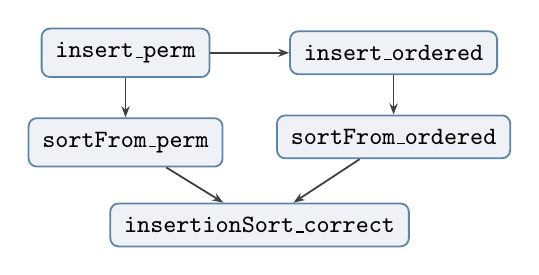
\begin{tikzpicture}[node distance=5mm and 10mm]
\node[module] (p) {\texttt{insert\_perm}};
\node[module,right=of p] (o) {\texttt{insert\_ordered}};
\node[module,below=of p] (pp) {\texttt{sortFrom\_perm}};
\node[module,below=of o] (oo) {\texttt{sortFrom\_ordered}};
\node[module,below=8mm of $(pp)!0.5!(oo)$] (end) {\texttt{insertionSort\_correct}};
\draw[dataflow](p)--(pp);\draw[dataflow](p)--(o);\draw[dataflow](o)--(oo);
\draw[dataflow](pp)--(end);\draw[dataflow](oo)--(end);
\end{tikzpicture}\end{center}
箭头从已知引理指向调用它的证明。横向那支箭头很重要：为了证明一次插入后仍有序，我们需要辨认插入后的某个元素从哪里来。排列引理可以告诉我们，它要么是新值，要么来自旧列表。
\par\smallskip{\footnotesize\href{https://yeyaozhi.eu.cc/learning/lean-lab/?lesson=insertion-spec\#proof}{打开本页对应的 Lean 实验}}
\clearpage\pdfbookmark[0]{一次插入怎样保住重复次数}{p12}\label{p12}\HandoutLesson{插入的第一个引理}{一次插入怎样保住重复次数}
固定待插入的 $x$，目标是 \src{(insert r x ys).Perm (x :: ys)}。右边把新牌直接放在最前面，给出了一个容易核对的参照。只要左边能由右边调换位置得到，就知道没有丢牌或多造牌。
\subhead{把一个具体交换拆开}
将 $4$ 插入 $[2,5]$ 会得到 $[2,4,5]$。参照是 $[4,2,5]$。先看尾部，把 $4$ 插入 $[5]$ 得到 $[4,5]$，已经等于尾部的参照。在两边都加回 $2$，得到 $[2,4,5]$；最后交换前两项，就到达整列的参照 $[4,2,5]$。
\subhead{读原证明的三个分支}
\begin{leanblock}
\lineofcode{1.0}{induction ys with}
\lineofcode{1.0}{| nil => exact .refl \_}
\lineofcode{1.0}{| cons y ys ih =>}
\lineofcode{2.0}{by\_cases h : r x y}
\lineofcode{2.0}{\ensuremath{\cdot} rw [insert, if\_pos h]}
\lineofcode{2.0}{\ensuremath{\cdot} rw [insert, if\_neg h]}
\lineofcode{3.0}{exact (List.Perm.cons y ih).trans (.swap x y ys)}
\end{leanblock}
空表时两边都是 $[x]$，\src{Perm.refl} 给出“自己是自己的排列”。非空时用比较结果分两支，\src{h} 在第一支证明 \src{r x y}，在第二支证明其否定。\src{if\_pos} 和 \src{if\_neg} 据此选中程序实际执行的分支。
比较成立时，输出本来就是 $x::y::ys$。比较失败时，输出形如 $y::\mathrm{insert}(x,ys)$。归纳假设 \src{ih} 说后面的插入结果与 $x::ys$ 互为排列。\src{Perm.cons y ih} 允许两边同时加上 $y$；\src{.swap} 交换两个相邻表头；\src{.trans} 把两段排列证明首尾接起来。
\HandoutBox{在纸上把“同时加表头”和“交换两个表头”各画一个箭头。只证明每个元素都出现过，会遗漏什么？试着拿含有两个 $2$ 的输入来反驳。}
\par\smallskip{\footnotesize\href{https://yeyaozhi.eu.cc/learning/lean-lab/?lesson=insertion-spec\#proof}{打开本页对应的 Lean 实验}}
\clearpage\pdfbookmark[0]{从一次比较推出整列有序}{p13}\label{p13}\HandoutLesson{插入的第二个引理}{从一次比较推出整列有序}
假设 $y::ys$ 已经有序。把这个假设拆开，可以拿到两件事：$y$ 排在尾部每个元素 $z$ 前面，满足 $r(y,z)$；尾部 \src{ys} 自身也有序。在代码中 \src{List.pairwise\_cons.mp hs} 取出这两件事，分别命名为 \src{hy} 和 \src{hys}。
\subhead{情形一：新值可以放在表头}
若 $r(x,y)$，输出就是 $x::y::ys$。旧的后半列仍有序。新增的任务只有“$x$ 能放在后面每个值之前”。遇到 $y$ 本身，刚才那次比较给出了证明；遇到 \src{ys} 中的 $z$，由 $r(x,y)$、$r(y,z)$ 和传递性推出 $r(x,z)$。因此比较表头一次就足够。
\begin{leanblock}
\lineofcode{0.0}{rw [insert, if\_pos hxy, List.pairwise\_cons]}
\lineofcode{0.0}{refine \ensuremath{\langle}?\_, hs\ensuremath{\rangle}}
\end{leanblock}
尖括号的第二格已经填入旧列的有序性 \src{hs}。\src{?\_} 留下第一格，要求我们逐个说明新表头与后面元素的关系。
\subhead{情形二：保留原来的表头}
若 $r(x,y)$ 为假，程序保留 $y$，在尾部递归插入 $x$。对较短列表使用归纳假设，可知新尾部有序。还需要验证 $y$ 能放在新尾部的每个 $z$ 前面。上页的排列引理保证 $z$ 的来历只有两种：
\begin{itemize}
\item 如果 $z=x$，全可比性给出 $r(x,y)\lor r(y,x)$。前一项已被排除，所以 $r(y,x)$ 成立。
\item 如果 $z$ 是旧尾部元素，原先的 \src{hy} 就给出 $r(y,z)$。
\end{itemize}
以 $x=4$、旧列 $[2,5]$ 为例，新尾部是 $[4,5]$。$2\le4$ 来自比较失配后的反向关系；$2\le5$ 来自原列表有序。两种依据各用一次。
\HandoutBox{现在可以给关系 r 写出三个接口要求：程序要能判定一次比较；证明需要传递性；比较失败后要能从全可比性选出反向关系。}
\par\smallskip{\footnotesize\href{https://yeyaozhi.eu.cc/learning/lean-lab/?lesson=insertion-order\#proof}{打开本页对应的 Lean 实验}}
\clearpage\pdfbookmark[0]{从一次插入走到任意长度的输入}{p14}\label{p14}\HandoutLesson{§2.1 · 完成规格}{从一次插入走到任意长度的输入}
\src{sortFrom r acc rest} 从已排部分 \src{acc} 开始，把 \src{rest} 中的元素逐个插入。我们要证明：任给有序的 \src{acc}，处理完 \src{rest} 所得的列表仍有序。对尚待处理的 \src{rest} 做归纳，初值 \src{acc} 仍可任选。
\begin{leanblock}
\lineofcode{1.0}{induction rest generalizing acc with}
\lineofcode{1.0}{| nil => exact hAcc}
\lineofcode{1.0}{| cons x xs ih =>}
\lineofcode{2.0}{have hStep : (insert r x acc).Pairwise r :=}
\lineofcode{3.0}{insert\_ordered r trans total x acc hAcc}
\lineofcode{2.0}{exact ih (insert r x acc) hStep}
\end{leanblock}
空表分支立即返回 \src{acc}，手里的 \src{hAcc} 正好证明它有序。在非空分支，\src{have} 给一个中间事实起名。调用上页的引理得到 \src{hStep} 后，当前目标依旧是最终结果有序。现在把更新后的累积列表和证明 \src{hStep} 一起交给 \src{ih}，剩余输入已经缩成 \src{xs}。
\subhead{另一条归纳线怎样保持全部元素}
若用 $\sim$ 表示“互为排列”，令 $a'=\mathrm{insert}(x,a)$。从 $a$ 出发处理 $x::s$ 等于从 $a'$ 出发处理 $s$。后者的结果按归纳假设与 $a'\mathbin{++}s$ 互为排列。一次插入的排列引理又告诉我们
\[
 a'\mathbin{++}s\ \sim\ (x::a)\mathbin{++}s\
 \sim\ a\mathbin{++}(x::s).
\]
第一步在一对排列的右边接上相同尾部；第二步让 $x$ 越过整段 $a$。源码用 \src{append\_right} 和 \src{perm\_middle} 的反向证明完成这两步。
\subhead{回到最外层的入口}
\begin{leanblock}
\lineofcode{1.0}{constructor}
\lineofcode{1.0}{\ensuremath{\cdot} exact sortFrom\_ordered r trans total xs [] .nil}
\lineofcode{1.0}{\ensuremath{\cdot} exact sortFrom\_perm r xs []}
\end{leanblock}
令初始累积列表为 $[]$。空表有序的证明是 \src{.nil}；空表拼上 \src{xs} 按定义就是 \src{xs}。两条子目标分别关闭，这就证明函数式插入排序对任意自然数列表满足完整规格。
\par\smallskip{\footnotesize\href{https://yeyaozhi.eu.cc/learning/lean-lab/?lesson=insertion-spec\#proof}{打开本页对应的 Lean 实验}}
\clearpage\pdfbookmark[0]{改为降序，哪些证明要重做}{p15}\label{p15}\HandoutLesson{第四版练习 2.1-3}{改为降序，哪些证明要重做}
把关系 $r(x,y)$ 定义为 $y\le x$。例如处理 $[2,5,2]$，第一次插入得到 $[2]$，第二次比较“$2\le5$？”成立，把 $5$ 放在前面。第三次遇到表头 $5$ 时测试“$5\le2$？”失败，于是继续比较尾部。最终 $[5,2,2]$ 有序，原来的两个 $2$ 都在。
\subhead{将一般定理用到一个具体关系}
源码中 \src{fun x y => y \ensuremath{\leq} x} 就是这个二元关系。目标仍由合取组成：按反向关系有序，而且结果与输入互为排列。\src{apply insertionSort\_correct} 把一般定理的结论对准当前目标。Lean 已经从目标推断出关系和列表，剩余两个条件要我们填写。
\begin{leanblock}
\lineofcode{1.0}{apply insertionSort\_correct}
\lineofcode{1.0}{\ensuremath{\cdot} intro x y z hyx hzy}
\lineofcode{2.0}{exact Nat.le\_trans hzy hyx}
\lineofcode{1.0}{\ensuremath{\cdot} intro x y}
\lineofcode{2.0}{exact Nat.le\_total y x}
\end{leanblock}
第一支要证明传递性。把一般关系的公式
\[
 r(x,y)\ \longrightarrow\ r(y,z)\ \longrightarrow\ r(x,z)
\]
逐项换成自然数关系，就得到“若 $y\le x$ 且 $z\le y$，则 $z\le x$”。为了让不等式的中间项接起来，先递给 \src{Nat.le\_trans} 的应是 $z\le y$，再给 $y\le x$。这就是代码里 \src{hzy hyx} 次序的来历。
第二支要求 $y\le x$ 或 $x\le y$。\src{Nat.le\_total y x} 的输出恰好匹配。一般定理里关于元素排列的证据也随之可用。
\HandoutBox{能把这里的 $\le$ 换成严格小于吗？让 $x=y=2$。这时 $x<y$ 和 $y<x$ 同时为假，全可比性无法通过。这个检查看出了重复元素带来的实际约束。}

\par\smallskip{\footnotesize\href{https://yeyaozhi.eu.cc/learning/lean-lab/?lesson=descending\#proof}{打开本页对应的 Lean 实验}}
\clearpage\pdfbookmark[0]{查找为什么返回 Option Nat}{p16}\label{p16}\HandoutLesson{第四版练习 2.1-4 · 执行}{查找为什么返回 Option Nat}
在 $[7,4,9]$ 里找 $4$，答案是下标 $1$。在同一个列表里找 $6$，没有可交回的合法下标。若用数字 $0$ 表示失败，便无法区别“没找到”和“在第一项找到”。\src{Option Nat} 提供两种构造：\src{none} 表示空缺，\src{some i} 保存一个自然数下标 $i$。
\begin{leanblock}
\lineofcode{0.0}{def linearSearch (key : Nat) : List Nat \ensuremath{\to} Option Nat}
\lineofcode{1.0}{| [] => none}
\lineofcode{1.0}{| x :: xs =>}
\lineofcode{2.0}{if x = key then some 0 else (linearSearch key xs).map Nat.succ}
\end{leanblock}
\subhead{为什么尾部的答案要加一}
从 $[7,4,9]$ 的表头开始，$7\ne4$，任务交给 $[4,9]$。在尾部看来，$4$ 就在位置 $0$，所以返回 \src{some 0}。回到原来的列表，它前面多了一个 $7$，下标要加一，得到 \src{some 1}。这里的 $1$ 是位置，目标值仍然是 $4$。
\src{Nat.succ} 把 $j$ 变成 $j+1$。\src{map} 把这个操作伸进 \src{Option} 的包装里。如果尾部给出 \src{some j}，那么整体得到 \src{some (j+1)}；如果尾部给出 \src{none}，加一操作没有对象，整体仍是 \src{none}。
\subhead{对两种返回值各问一句}
\[
\begin{aligned}
\mathrm{search}(k,L)=\mathrm{none}
   &\iff k\notin L,\\
\mathrm{search}(k,L)=\mathrm{some}(i)
   &\implies L[i]?=\mathrm{some}(k).
\end{aligned}
\]
\src{xs[i]?} 是可失败的下标访问，越界时同样返回 \src{none}。第二式因此同时说明返回的位置存在，那里存放的确实是目标值。接下来两页分别证明这两句话。
\HandoutBox{先推算 \src{linearSearch 9 [7,4,9]} 的返回过程：最内层找到时是多少？回到上一层、再上一层各是多少？对 \src{linearSearch 8 [7,4,9]} 重做一次。}
\par\smallskip{\footnotesize\href{https://yeyaozhi.eu.cc/learning/lean-lab/?lesson=search\#proof}{打开本页对应的 Lean 实验}}
\clearpage\pdfbookmark[0]{把“找不到”证明成双向等价}{p17}\label{p17}\HandoutLesson{第四版练习 2.1-4 · 缺失}{把“找不到”证明成双向等价}
令 $F(L)$ 表示查找返回 \src{none}，令 $A(L)$ 表示目标值不在列表 $L$。我们要证明 $F(L)\leftrightarrow A(L)$。正向保证程序报告失败时列表里确实没有，反向保证列表里没有时程序会报告失败。
\begin{leanblock}
\lineofcode{0.0}{theorem linearSearch\_none\_iff (key : Nat) (xs : List Nat) :}
\lineofcode{2.0}{linearSearch key xs = none \ensuremath{\leftrightarrow} key \ensuremath{\notin} xs := by}
\lineofcode{1.0}{induction xs with}
\lineofcode{1.0}{| nil => simp [linearSearch]}
\lineofcode{1.0}{| cons x xs ih =>}
\lineofcode{2.0}{by\_cases hx : x = key}
\lineofcode{2.0}{\ensuremath{\cdot} simp [linearSearch, hx]}
\lineofcode{2.0}{\ensuremath{\cdot} simpa [linearSearch, hx, Ne.symm hx] using ih}
\end{leanblock}
\subhead{空表、表头命中、表头失配}
空表时，左边从定义化成 \src{none = none}，右边说明空列表没有成员，两边都成立。若表头等于目标值，函数返回 \src{some 0}，左边为假；目标就在表头，右边也为假。这里要证明的是等价关系，两边都为假时，这个等价关系为真。
若表头失配，剩下的目标读作：
\[
\underbrace{\text{尾部结果经下标加一后仍为空}}_{\iff F(xs)}
\ \longleftrightarrow\
\underbrace{\text{目标既不是表头，也不在尾部}}_{\iff A(xs)}.
\]
左边用上页的 \src{map} 两条计算规则。右边用“属于 $x::xs$ 等价于等于 $x$ 或属于 \src{xs}”以及 $x\ne key$。因此要交出的命题正是已有的 \src{ih}。
\subhead{最后一行浓缩了哪些依据}
\src{simpa [...] using ih} 会按给定规则化简眼下的目标和已有事实，再检查它们能否对上。比较是 \src{x = key}，成员关系展开时也可能出现 \src{key = x}。\src{Ne.symm hx} 提供失配条件的反方向，避免这两个写法对不上。
\HandoutBox{在纸上对 $[]$、$[4]$、$[7,4]$ 分别判断等价式的左右两边。会有一组“两边都假”；尝试说出为什么它仍然通过定理的检查。}
\par\smallskip{\footnotesize\href{https://yeyaozhi.eu.cc/learning/lean-lab/?lesson=search\#proof}{打开本页对应的 Lean 实验}}
\clearpage\pdfbookmark[0]{返回的下标为什么一定正确}{p18}\label{p18}\HandoutLesson{第四版练习 2.1-4 · 命中}{返回的下标为什么一定正确}
假设 \src{found : linearSearch key xs = some i}。目标是 \src{xs[i]? = some key}。我们手里已经有“程序给了下标”的前提，要用它排除不可能的执行路径。分支越多，越值得先写一张表。
\begin{center}\small\begin{tabularx}{\linewidth}{@{}l>{\raggedright\arraybackslash}X>{\raggedright\arraybackslash}X@{}}\toprule
输入与比较 & 程序输出 & 从 found 得到什么\\\midrule
空列表 & \src{none} & 与 \src{some i} 冲突，此支不可能。\\
表头命中 & \src{some 0} & 必有 $i=0$；下标 $0$ 处就是目标值。\\
表头失配，尾部失败 & \src{none} & 又与 found 冲突。\\
表头失配，尾部命中 $j$ & \src{some (j+1)} & $i=j+1$，用尾部位置 $j$ 的归纳假设。\\\bottomrule\end{tabularx}\end{center}
\subhead{在最难的一支中追到底}
\src{cases ht : linearSearch key xs with} 拆开尾部的返回值，并把它的取值记录在等式 \src{ht} 中。假设尾部返回 \src{some j}。将 \src{ht} 和失配条件代入 \src{found}，已知 \src{some (j+1) = some i}，于是 $j+1=i$。源码里的 \src{simp [...] at found} 把这些计算用在已知条件上，\src{subst i} 随后在相关表达式中替换 $i$。
此时整个列表是 $x::xs$。读取它的第 $j+1$ 项，按定义就是读尾部 \src{xs} 的第 $j$ 项。对尾部使用 \src{ih j ht}，已得 \src{xs[j]? = some key}，正是所需。
\subhead{用具体数字检验一次位置换算}
在 $[7,4,9]$ 找 $4$ 时，这个分支中 $x=7$，尾部为 $[4,9]$，$j=0$。尾部的第 $0$ 项是 $4$，因此整个列表的第 $1$ 项也是 $4$。若忘了给尾部返回值加一，函数会声称下标 $0$ 处是 $4$，实际那里是 $7$。这条反例能准确定位程序应修改的地方。
\HandoutBox{两个查找定理合起来保证命中与缺失都可信。若还要单独证明“返回重复值的最小下标”，规格还需加入所有更小位置均不匹配的条件。}
\par\smallskip{\footnotesize\href{https://yeyaozhi.eu.cc/learning/lean-lab/?lesson=search\#proof}{打开本页对应的 Lean 实验}}
\clearpage\pdfbookmark[0]{六道题，把纸上的推理写进 Lean}{p19}\label{p19}\HandoutLesson{自测 · 先独立完成}{六道题，把纸上的推理写进 Lean}
先在纸上作答。第 1–3 题可以在在线编辑器中新开文件，第一行写 \src{import Std}；本页给出定理的名字和目标，参考证明在下一页。第 4–6 题需要解释算法的状态，建议保留中间计算。
\subhead{1　构造与取出}
已知 \src{h : (P \ensuremath{\wedge} Q) \ensuremath{\wedge} R}，要求得到 \src{R \ensuremath{\wedge} Q}。先写出 \src{constructor} 后的两个目标，再分别用 \src{exact} 填上。特别留意 $Q$ 藏在括号的哪一层。
\subhead{2　把等式用到假设中}
已知 \src{h : a = b} 和 \src{ha : a + 1 = 9}，目标是 \src{b + 1 = 9}。这次试着保留目标的写法，改写 \src{ha}，再交出改写过的假设。预先写出替换之前和之后 \src{ha} 各是什么类型。
\subhead{3　用自己的递归函数数元素}
\begin{leanblock}
\lineofcode{0.0}{def countItems : List Nat \ensuremath{\to} Nat}
\lineofcode{1.0}{| [] => 0}
\lineofcode{1.0}{| \_ :: xs => countItems xs + 1}
\end{leanblock}
在任意列表 \src{xs} 上证明 \src{countItems (xs ++ []) = countItems xs}。先尝试仅用第 7 页的引理，再试一次不调用该引理、直接归纳的证明。两种方法分别把哪一步留给了 Lean？
\subhead{4　修复一个太弱的归纳假设}
输入是整数列表 $[-3,5]$，累加器初值是 $0$。请分别写下第一、二次递归调用的参数，以及下一次应调用的归纳假设。如果证明中把初值锁死在 $0$，第一次卡在哪个式子？
\subhead{5　一轮插入的两张收据}
把 $3$ 插入 $[1,3,4]$。写下完整结果，指出至少一个重复值。在表头 $1$ 选择“继续递归”的分支时，为证明表头能排在新尾部前面，你需要说明新尾部元素的哪两种来历？
\subhead{6　只测是否缺失够不够}
某人修改了线性查找：如果目标出现，总返回 \src{some 0}；否则返回 \src{none}。这个函数能通过第 17 页的缺失规格吗？给出长度尽量短的输入，让第 18 页的下标规格失败。
\clearpage\pdfbookmark[0]{前三题的可运行证明}{p20}\label{p20}\HandoutLesson{自测 · 参考解答}{前三题的可运行证明}
\subhead{1　让目标决定取哪一个投影}
\begin{leanblock}
\lineofcode{0.0}{example (P Q R : Prop) (h : (P \ensuremath{\wedge} Q) \ensuremath{\wedge} R) : R \ensuremath{\wedge} Q := by}
\lineofcode{1.0}{constructor}
\lineofcode{1.0}{\ensuremath{\cdot} exact h.right}
\lineofcode{1.0}{\ensuremath{\cdot} exact h.left.right}
\end{leanblock}
第一项目标是 $R$，位于外层右侧。第二项目标是 $Q$，先从外层向左取出 $P\wedge Q$，再向右取出 $Q$。若把两个分支的答案交换，第一处就会出现类型不匹配。
\subhead{2　改写已知条件}
\begin{leanblock}
\lineofcode{0.0}{example (a b : Nat) (h : a = b) (ha : a + 1 = 9) :}
\lineofcode{2.0}{b + 1 = 9 := by}
\lineofcode{1.0}{rw [h] at ha}
\lineofcode{1.0}{exact ha}
\end{leanblock}
\src{at ha} 选定已知条件作为重写位置。$a+1=9$ 变成 $b+1=9$，因此现在的 \src{ha} 与目标相同。另一种写法是在目标中用 \src{rw [\ensuremath{\leftarrow} h]}，再使用原来的 \src{ha}。
\subhead{3　复用引理，或者重新归纳}
把第 19 页的 \src{countItems} 和第 7 页的 \src{appendNil} 放在同一命名空间后，第一种证明只需 \src{rw [appendNil xs]}，它把函数的输入替换为 \src{xs}。第二种写成：
\begin{leanblock}
\lineofcode{0.0}{example (xs : List Nat) : countItems (xs ++ []) = countItems xs := by}
\lineofcode{1.0}{induction xs with}
\lineofcode{1.0}{| nil => rfl}
\lineofcode{1.0}{| cons x rest ih =>}
\lineofcode{2.0}{change countItems (rest ++ []) + 1 = countItems rest + 1}
\lineofcode{2.0}{rw [ih]}
\end{leanblock}
这里先用定义把“数一个非空表”展开成“数尾部再加一”。$+1$ 在两边都保留，归纳假设替换的是内部的计数。比较第 7 页的证明：那里两边相同的是表头，这里两边相同的是加一操作。
\clearpage\pdfbookmark[0]{后三题与独立读证明的方法}{p21}\label{p21}\HandoutLesson{自测 · 参考解答}{后三题与独立读证明的方法}
\subhead{4　初值要能跟着程序一起改变}
从 \src{sumFrom 0 [-3,5]} 开始，下一次是 \src{sumFrom (-3) [5]}，再下一次是 \src{sumFrom 2 []}。第一步推理需要把适用于尾部 $[5]$ 的归纳假设用在初值 $-3$ 上。若只知道 \src{sumFrom 0 [5] = [5].sum} 的数学内容，等式左侧不能与当前调用匹配。把初值推广后，$-3+5=2$，随后空表直接返回 $2$。
\subhead{5　把来历与顺序分别核对}
先保留 $1$，对 $[3,4]$ 递归插入 $3$。$3\le3$ 成立，于是新尾部变成 $[3,3,4]$，最终结果是 $[1,3,3,4]$。一次插入的排列引理保证新尾部成员要么是新插入的 $3$，要么来自旧尾部 $[3,4]$。第一种用 $1\le3$；第二种用旧列的有序性。值相同可能同时满足两种描述，这不会妨碍分情况证明。
\subhead{6　把错误放进能发现它的规格}
按题设，程序恰在目标缺失时返回 \src{none}，所以通过缺失规格。取列表 $[7,4]$ 和目标 $4$。它返回 \src{some 0}，而 $[7,4][0]$ 是 $7$。在长度为零或一的列表中，若找到目标，唯一可行的位置就是 $0$，因此长度二已经是最短反例。
\subhead{下一次打开一个陌生定理}
先把定理翻成“任给哪些对象、另需哪些假设、最终保证什么”。给它挑一个最小的正例和一个能暴露缺失条件的反例。随后对着源码只读当前一行：这一行引用的证明来自哪里？它的结论是否与当前目标对得上？遇到递归或归纳，多问一句“哪个参数真的变小了，哪个参数下次会改变”。
\HandoutBox{闭卷验收：能用自己的话解释「只证明有序还差什么」「为何要 generalizing acc」「为何查找的 some 分支需要加一」，再回到实验室逐行预测目标。}
\clearpage\pdfbookmark[0]{课程、定理与查阅入口}{p22}\label{p22}\HandoutLesson{索引 · 回到源码}{课程、定理与查阅入口}
\begin{tabularx}{\linewidth}{@{}l>{\raggedright\arraybackslash}Xr@{}}\toprule
源文件 & 定理、定义或程序状态 & 页\\\midrule
Foundations & \src{swapAnd}，引入、拆分与两个投影 & 2–4\\
& \src{addOneEq}，重写方向、自反性 & 5\\
& \src{appendNil}，列表拼接、结构归纳 & 6–7\\
SumAndSearch & \src{sumFrom}, \src{sumFrom\_correct}, \src{sumList\_correct}，累加器与结合律 & 8–9\\
InsertionSort & \src{insert}, \src{sortFrom}, \src{insertionTraceFrom}, \src{insertionTrace}，一次插入与逐轮状态 & 10\\
& \src{insert\_perm}, \src{insert\_ordered}，排列与有序性的保持 & 11–13\\
& \src{sortFrom\_ordered}, \src{sortFrom\_perm}, \src{insertionSort}, \src{insertionSort\_correct} & 14\\
& \src{descending\_correct}，传递性与全可比性 & 15\\
SumAndSearch & \src{linearSearch}, \src{linearSearch\_none\_iff}, \src{linearSearch\_sound} & 16–18\\\bottomrule\end{tabularx}
\subhead{版本、模型与资料}
第 1–22 页对照站内三个同名 \src{.lean} 文件，使用 Lean 4.28.0 和其标准库。新增练习的可运行解答可在阅读器下载。阅读器展示的讲义页与下载 PDF 的页码一致。
前篇对照《算法导论》第四版 §2.1，原书以数组讲插入排序。本讲义用自然数列表证明排序和查找，用整数列表证明求和；插入排序处理的是结果有序性和元素保留。数组下标的内存操作、时间界和稳定性需要各自的规格。书中的练习号用于定位主题，书目与配套资源见 \href{https://mitpress.mit.edu/9780262046305/introduction-to-algorithms/}{MIT Press 第四版书页}。
可在 \href{https://yeyaozhi.eu.cc/learning/lean-lab/}{Lean 实验室} 调出 8 节交互课，或从 \href{https://tanktechnology.github.io/CLRS-Lean/}{CLRS-Lean 章节导读} 查阅更多选定算法。策略和证明项的关系可读 Lean 官方教材 \href{https://lean-lang.org/theorem_proving_in_lean4/Tactics/}{Tactics}；列表归纳的原理见 \href{https://lean-lang.org/theorem_proving_in_lean4/Induction-and-Recursion/}{Induction and Recursion}。
% BEGIN FOURTH EDITION CHAPTER TWO CONTINUATION
\clearpage\pdfbookmark[0]{2.1-5 · 把最后一次进位也写下来}{p23}\label{p23}\HandoutLesson{第四版 · 2.1-5}{把最后一次进位也写下来}
在纸上写 $1101_2+0111_2$。先盖住最左边三列，只看个位的 $1+1$。这一列应写 $0$，再把一个 $1$ 送到下一列。现在逐列填写表格；表中的行序就是程序读取输入的顺序。
\begin{center}\begin{tabular}{ccccccc}\toprule 位 $i$ & $a_i$ & $b_i$ & 传入 $c$ & 合计 & 写下 $s_i$ & 传出 $c'$\\\midrule
0&1&1&0&2&0&1\\1&0&1&1&2&0&1\\2&1&1&1&3&1&1\\3&1&0&1&2&0&1\\\bottomrule\end{tabular}\end{center}
程序先得到低位在前的 $[0,0,1,0]$。此时手里还有进位 $1$，附在末尾，结果是 $[0,0,1,0,1]$。按通常的高位在前写成 $10100_2=20$，等于 $13+7$。若把空输入分支写成空列表，最后的十六就会丢掉。
\subhead{把一行表变成一个定理}
\begin{leanblock}
\lineofcode{0.0}{def bitSum (a b c : Bool) := xor (xor a b) c}
\end{leanblock}
\begin{leanblock}
\lineofcode{0.0}{def carry (a b c : Bool) := (a \&\& b) || (a \&\& c) || (b \&\& c)}
\end{leanblock}
\begin{leanblock}
\lineofcode{0.0}{theorem column (a b c : Bool) :}
\lineofcode{1.8}{(bitSum a b c).toNat + 2 * (carry a b c).toNat = a.toNat + b.toNat + c.toNat := by}
\lineofcode{0.9}{cases a <;> cases b <;> cases c <;> decide}
\end{leanblock}
\src{Bool} 只有两个值，对应位 $0,1$。\src{bitSum} 用三位异或取奇偶性，\src{carry} 检查三位中是否至少有两位为真。上面等号左边把传出的进位乘二，它将在高一位起作用。三个 \src{cases} 形成 $2^3=8$ 个分支；\src{<;>} 把后面的策略用于每一支。每支都只剩具体数的等式，由 \src{decide} 检查。
\HandoutBox{自己填 $1+0+1$ 和 $1+1+1$ 两行。两行都进位，留下的低位为什么不同？}
\par\smallskip{\footnotesize\href{https://yeyaozhi.eu.cc/assets/lean-handout/BinaryAndCosts.lean}{本页 Lean 源码 · \texttt{BinaryAndCosts.lean}}}
\clearpage\pdfbookmark[0]{2.1-5 · 从一列的等式拼出整串的等式}{p24}\label{p24}\HandoutLesson{第四版 · 2.1-5}{从一列的等式拼出整串的等式}
把第一行划掉。原来尚未计算的两段对应 $110_2$ 和 $011_2$，进入尾部的进位是 $1$。它们合起来是 $6+3+1=10$；乘二再加刚写的低位 $0$，得到 $20$。归纳步就是把这个算式里的具体数换成任意尾部。
\begin{leanblock}
\lineofcode{0.0}{def addBits : List (Bool \ensuremath{\times} Bool) \ensuremath{\to} Bool \ensuremath{\to} List Bool}
\lineofcode{0.9}{| [], c => [c]}
\lineofcode{0.9}{| (a,b) :: xs, c => bitSum a b c :: addBits xs (carry a b c)}
\end{leanblock}
输入是成对的位列，因此两个数的位宽天然相同。\src{value} 对空列表取零，对表头 $a$ 和尾部 $A$ 取 $a+2\,\mathrm{value}(A)$。若把函数限制在初始进位 $0$，第一次递归很可能就用不上归纳假设，所以正确性定理允许任意进位 $c$。
\begin{leanblock}
\lineofcode{0.0}{theorem addBits\_correct (xs : List (Bool \ensuremath{\times} Bool)) (c : Bool) :}
\lineofcode{1.8}{value (addBits xs c) = value (xs.map Prod.fst) + value (xs.map Prod.snd) + c.toNat := by}
\lineofcode{0.9}{induction xs generalizing c with}
\lineofcode{0.9}{| nil => simp [addBits, value]}
\lineofcode{0.9}{| cons p xs ih =>}
\lineofcode{1.8}{obtain \ensuremath{\langle}a,b\ensuremath{\rangle} := p}
\lineofcode{1.8}{simp only [List.map\_cons, addBits, value, ih]}
\lineofcode{1.8}{have h := column a b c}
\lineofcode{1.8}{omega}
\end{leanblock}
\src{generalizing c} 保留任选进位的权利。空表时返回单独的 $c$。非空时 \src{obtain} 拆开这一列的两个输入位；\src{map Prod.fst}、\src{map Prod.snd} 分别读每列的第一、第二分量。\src{simp only} 依次展开表头和赋值规则，再把下一层的结果按归纳假设替换。写 $A,B$ 为两条尾部的值，剩余等式是
\[
 s+2(A+B+c')=(a+2A)+(b+2B)+c .
\]
\src{have h} 提供 $s+2c'=a+b+c$，\src{omega} 整理整数系数，把左右两式对齐。独立的 \src{addBits\_width} 对每多一列就在输出前多放一位，基例输出一位，所以恰好输出 $n+1$ 位，即使最高进位是零也保留它。
\par\smallskip{\footnotesize\href{https://yeyaozhi.eu.cc/assets/lean-handout/BinaryAndCosts.lean}{本页 Lean 源码 · \texttt{BinaryAndCosts.lean}}}
\clearpage\pdfbookmark[0]{2.2-1 · 给三次函数找到两道界}{p25}\label{p25}\HandoutLesson{第四版 · 2.2-1}{给三次函数找到两道界}
取 $n=10$，原函数四项分别为 $1,10000,-1000,3$，和为 $9004$。这时候二次项远大于三次项。要回答增长阶，应找到从某处起始终成立的上下界，不能只看这个输入。
\subhead{把分母先移走}
令 $F(n)=1000 f(n)=n^3+100000n^2-100000n+3000$。固定 $n\ge1$。因为 $n^2-n\ge0$，所以 $F(n)\ge n^3$。求上界时丢掉负项，再用 $n^2\le n^3$ 和 $1\le n^3$，得到 $F(n)\le103001n^3$。两边除以正数 $1000$，便给出了 $\Theta(n^3)$ 所需的两个正常数及起点 $n_0=1$。
\begin{leanblock}
\lineofcode{0.0}{theorem cubic (n : Int) (hn : 1 \ensuremath{\leq} n) :}
\lineofcode{1.8}{n\textasciicircum{}3 \ensuremath{\leq} scaled n \ensuremath{\wedge} scaled n \ensuremath{\leq} 103001*n\textasciicircum{}3 := by}
\lineofcode{0.9}{have h\ensuremath{{}_{2}} : n \ensuremath{\leq} n\textasciicircum{}2 := by}
\lineofcode{1.8}{simpa [Int.pow\_succ] using Int.mul\_le\_mul\_of\_nonneg\_left hn (show 0 \ensuremath{\leq} n by omega)}
\lineofcode{0.9}{have h\ensuremath{{}_{3}} : n\textasciicircum{}2 \ensuremath{\leq} n\textasciicircum{}3 := by}
\lineofcode{1.8}{simpa only [Int.mul\_one, Int.pow\_succ n 2] using Int.mul\_le\_mul\_of\_nonneg\_left hn (show 0 \ensuremath{\leq} n\textasciicircum{}2 by omega)}
\lineofcode{0.9}{unfold scaled}
\lineofcode{0.9}{omega}
\end{leanblock}
\src{Int} 允许直接处理减号。两条 \src{have} 分别给出 $n\le n^2$ 与 $n^2\le n^3$。它们都从 $1\le n$ 出发，同乘非负的 $n$ 或 $n^2$；\src{simpa} 把结果写成幂。\src{unfold} 替换 $F$ 的定义。最后 \src{omega} 把已经建立的幂之间的不等式相加，此时不用它猜测乘法的单调性。
\HandoutBox{上界系数可以很松。若只证明 $f(n)\le Cn^3$，还缺哪一半？例如 $n^2$ 同样满足这句上界。}
\par\smallskip{\footnotesize\href{https://yeyaozhi.eu.cc/assets/lean-handout/BinaryAndCosts.lean}{本页 Lean 源码 · \texttt{BinaryAndCosts.lean}}}
\clearpage\pdfbookmark[0]{2.2-2 · 选择排序每一轮固定哪个位置}{p26}\label{p26}\HandoutLesson{第四版 · 2.2-2}{选择排序每一轮固定哪个位置}
用 $[4,2,1,3]$ 手算。第一轮扫描四项找出 $1$，与首项 $4$ 交换，成为 $[1\mid 2,4,3]$。第二轮最小值 $2$ 就在待处理部分的首位，得到 $[1,2\mid 4,3]$。第三轮交换 $4,3$。只剩一个数时，没有任何次序需要再决定。
\subhead{写成循环}
\begin{leanblock}
\lineofcode{0.0}{for i = 1 .. n-1}
\lineofcode{0.9}{j = i}
\lineofcode{0.9}{for t = i+1 .. n}
\lineofcode{1.8}{if A[t] < A[j] then j = t}
\lineofcode{0.9}{swap A[i], A[j]}
\end{leanblock}
内层每看完一个位置，$j$ 指向已扫描范围中的一个最小值。外层第 $i$ 轮前，前 $i-1$ 项有序，且其中每项不大于剩余的任一项；整个数组仍是输入的排列。开始时前缀为空。选出最小值并交换后，旧前缀可以安全地接上它，余下的每项仍不小于它。交换保留元素的次数。这三件事一起解释了停止时的完整规格。
\begin{leanblock}
\lineofcode{0.0}{def select : Pass := fun a xs =>}
\lineofcode{0.9}{let m := (a::xs).min (by simp)}
\lineofcode{0.9}{if m = a then (a,xs) else (m,replaceFirst m a xs)}
\end{leanblock}
\src{a} 是首项，\src{xs} 是它后面的部分。非空列表可取 \src{min}。若最小值已在首位，原样返回；否则把右侧第一次出现的最小值换成旧首项，再把最小值放到首位。比如第一轮是把尾部 $[2,1,3]$ 改为 $[2,4,3]$。这正是数组交换在列表上的效果，重复最小值也只换一个。
\par\smallskip{\footnotesize\href{https://yeyaozhi.eu.cc/assets/lean-handout/SortingPasses.lean}{本页 Lean 源码 · \texttt{SortingPasses.lean}}}
\clearpage\pdfbookmark[0]{2.2-2 · 选择排序的证据与比较次数}{p27}\label{p27}\HandoutLesson{第四版 · 2.2-2}{选择排序的证据与比较次数}
试着先排序 $[1,2,3,4]$。第一轮仍要拿首项与三项比较，后两轮各比较两次、一次。换成 $[4,3,2,1]$，交换变多，找最小值仍花 $3+2+1=6$ 次比较。
\subhead{Lean 如何拼接一次选择的证明}
\begin{leanblock}
\lineofcode{0.9}{intro a xs}
\lineofcode{0.9}{let m := (a::xs).min (by simp)}
\lineofcode{0.9}{have hm : (a::xs).min? = some m := List.min?\_eq\_some\_min (by simp)}
\lineofcode{0.9}{obtain \ensuremath{\langle}hmIn, low\ensuremath{\rangle} := List.min?\_eq\_some\_iff.mp hm}
\end{leanblock}
\src{hm} 把最小值函数的可选结果与这里的 $m$ 对接。\src{obtain} 从库定理取出两份事实：$m$ 确实出现过；它小于等于旧列表的每个元素。接下来 \src{by\_cases eq : m=a} 分两支。相等时排列用自反性；不等时由 $m$ 属于整列推出它属于尾部，用 \src{exchange} 证明交换前后为排列。最后通过排列的 \src{mem\_iff} 把新尾部的成员送回旧列，再应用最小值的下界。
通用定理 \src{rounds\_ok} 只向每轮索取“保持排列”和“选出的表头不大于新尾部”。令轮数 $k=n-1$。证明对 $k$ 归纳；$k=0$ 时条件 $n\le k+1$ 表明最多只剩一项。递推时，一轮排列的长度等式保证尾部恰好短一项，把归纳假设用于尾部，最后在它前面接上最小值。
\subhead{从六次比较推广到任意长度}
在 \src{BinaryAndCosts.lean} 中，\src{tri 0 = 0}，\src{tri (n+1) = tri n + n}。对 $n$ 归纳得 $2\,\mathrm{tri}(n)+n=n^2$。归纳步只需把左侧改写成 $2\mathrm{tri}(n)+2n+n+1$，再使用旧等式。于是比较总数是 $n(n-1)/2$。当 $n\ge2$ 时它介于 $n^2/4$ 和 $n^2/2$ 之间，最好、最坏均为 $\Theta(n^2)$。
\par\smallskip{\footnotesize\href{https://yeyaozhi.eu.cc/assets/lean-handout/SortingPasses.lean}{本页 Lean 源码 · \texttt{SortingPasses.lean}}}
\clearpage\pdfbookmark[0]{2.2-3 · 线性查找平均要看几项}{p28}\label{p28}\HandoutLesson{第四版 · 2.2-3}{线性查找平均要看几项}
纸上放四张不同的牌 $[8,3,6,2]$。抽到哪一个值，就从左边开始找它。四个目标等可能，查找次数分别是 $1,2,3,4$，总数 $10$，平均 $10/4=2.5$。这个小数是很多次查找的平均，一次具体查找永远只检查整数项。
\begin{leanblock}
\lineofcode{0.0}{def totalProbes : Nat \ensuremath{\to} Nat}
\lineofcode{0.9}{| 0 => 0}
\lineofcode{0.9}{| n+1 => totalProbes n + (n+1)}
\end{leanblock}
\begin{leanblock}
\lineofcode{0.0}{theorem successful\_sum (n : Nat) : 2 * totalProbes n = n*(n+1) := by}
\lineofcode{0.9}{induction n with}
\lineofcode{0.9}{| zero => rfl}
\lineofcode{0.9}{| succ n ih => simp only [totalProbes]; grind}
\end{leanblock}
\src{totalProbes} 累加所有可能命中位置的代价，而非在一次查找里走遍所有位置。列表多一项，新增的那种成功查找恰好花 $n+1$ 次。证明不在自然数里做会截断的小数除法，先证明 $2S(n)=n(n+1)$。\src{induction} 给出旧总数的等式，\src{simp only} 展开一次递推，\src{grind} 展开乘积，用旧等式消去 $2S(n)$。
\subhead{最后再取平均}
在 $n>0$、目标的唯一命中位置均匀分布时，平均为 $S(n)/n=(n+1)/2$。它夹在 $n/2$ 与 $n$ 之间，所以平均为 $\Theta(n)$。把目标放到最后一项，恰好检查 $n$ 次；任何输入至多检查 $n$ 次，最坏也为 $\Theta(n)$。
\HandoutBox{若允许查找失败，失败时要扫完整表；若有重复值，程序可能在抽到的位置之前就已命中。先说清概率模型，才能决定上述平均式是否适用。}
\par\smallskip{\footnotesize\href{https://yeyaozhi.eu.cc/assets/lean-handout/BinaryAndCosts.lean}{本页 Lean 源码 · \texttt{BinaryAndCosts.lean}}}
\clearpage\pdfbookmark[0]{2.2-4 · 给排序加上有序输入的快速返回}{p29}\label{p29}\HandoutLesson{第四版 · 2.2-4}{给排序加上有序输入的快速返回}
检查 $[2,2,5,8]$。依次比较相邻的 $2\le2$、$2\le5$、$5\le8$，全部通过，可直接交回输入。改成 $[2,5,2,8]$，第二次就看见 $5>2$，此时改走原来的排序程序。
\begin{leanblock}
\lineofcode{0.0}{def ordered : List Nat \ensuremath{\to} Bool}
\lineofcode{0.9}{| a :: b :: xs => decide (a \ensuremath{\leq} b) \&\& ordered (b :: xs)}
\lineofcode{0.9}{| \_ => true}
\end{leanblock}
\begin{leanblock}
\lineofcode{0.9}{unfold guarded}
\lineofcode{0.9}{split}
\lineofcode{0.9}{next h => exact \ensuremath{\langle}(ordered\_spec xs).mp h, .refl \_\ensuremath{\rangle}}
\lineofcode{0.9}{next => exact ok xs}
\end{leanblock}
前一段递归只把窗口向右移一项。\src{\&\&} 要求当前相邻对通过且剩余部分也通过，长度为零或一时直接通过。证明 \src{ordered\_spec} 的递推步要解释“相邻有序怎样推出整列有序”：从 $a\le b$ 和 $b$ 小于等于尾部每个 $z$，用传递性得到 $a\le z$。反向则从整列有序取出相邻对，再取出尾部有序。
后一段是包装函数的证明体。\src{unfold} 展开预检，\src{split} 按检查结果分支。成功分支用 \src{ordered\_spec} 取得有序证据，用 \src{.refl} 证明输入是自己的排列；失败分支把输入交给原排序的规格 \src{ok}。因此提前返回保留了原来的正确性。
\subhead{最好情形花多少}
有序输入上恰做 $n-1$ 次相邻比较，按单位代价为 $\Theta(n)$。在比较排序模型下，即便输入已经有序，也要获得足够证据：若 $n$ 个不同元素之间的比较图仍不连通，就不能排除某个分量的值整体落到另一个分量的另一侧。连通至少需要 $n-1$ 条边。预检因此达到了线性最好时间。
\par\smallskip{\footnotesize\href{https://yeyaozhi.eu.cc/assets/lean-handout/BinaryAndCosts.lean}{本页 Lean 源码 · \texttt{BinaryAndCosts.lean}}}
\clearpage\pdfbookmark[0]{2.3-1 · 八个数的归并树}{p30}\label{p30}\HandoutLesson{第四版 · 2.3-1}{八个数的归并树}
先分后并。抄下题给的八个数，把纸对折三次。下面每一行都保留了原来的相邻分组；归并时只在两队的队首之间做选择。
\[
\begin{aligned}
 &[3,41,52,26]\mid[38,57,9,49]\\
 &[3,41]\mid[52,26]\mid[38,57]\mid[9,49]\\
 &[3]\mid[41]\mid[52]\mid[26]\mid[38]\mid[57]\mid[9]\mid[49]\\[2pt]
 &\longrightarrow [3,41]\mid[26,52]\mid[38,57]\mid[9,49]\\
 &\longrightarrow [3,26,41,52]\mid[9,38,49,57]\\
 &\longrightarrow [3,9,26,38,41,49,52,57].
\end{aligned}
\]
最后一轮先比 $3,9$，取 $3$；再比 $26,9$，取 $9$；随后从 $26,38$ 取 $26$，从 $41,38$ 取 $38$。依次取 $41,49,52$ 后，左队为空，直接接上 $57$。
\subhead{用可核对的等式记录答案}
\begin{leanblock}
\lineofcode{0.0}{example : ([3,41,52,26,38,57,9,49] : List Nat).mergeSort}
\lineofcode{1.8}{= [3,9,26,38,41,49,52,57] := by}
\lineofcode{0.9}{simp +decide [List.mergeSort, List.MergeSort.Internal.splitInTwo,}
\lineofcode{1.8}{List.splitAt\_eq]}
\end{leanblock}
\src{List.mergeSort} 指定要运行的函数。\src{splitInTwo} 和 \src{splitAt\_eq} 让化简器看见具体怎么对半拆。\src{simp +decide} 针对这些具体自然数消解比较并核对列表相等。本题问一组确定输入，所以这一条计算证明回答了走查题；所有有序输入的归并正确性放在 2.3-3 证明。
\HandoutBox{不看最后两行，自己写出左半边四个数归并时的比较次序。若某一边先用尽，接上另一边时还需逐对比较吗？}
\par\smallskip{\footnotesize\href{https://yeyaozhi.eu.cc/assets/lean-handout/SearchAndMerge.lean}{本页 Lean 源码 · \texttt{SearchAndMerge.lean}}}
\clearpage\pdfbookmark[0]{2.3-2 · 递归会不会制造空区间}{p31}\label{p31}\HandoutLesson{第四版 · 2.3-2}{递归会不会制造空区间}
取闭区间 $[3,7]$。中点取整为 $5$，两个子区间是 $[3,5]$ 与 $[6,7]$，都非空。再试最窄的可分区间 $[6,7]$：中点是 $6$，两边各剩一个元素。此时两个端点相等，停止递归。
\begin{leanblock}
\lineofcode{0.0}{theorem split\_bounds (p r : Nat) (h : p < r) :}
\lineofcode{1.8}{p \ensuremath{\leq} (p+r)/2 \ensuremath{\wedge} (p+r)/2 < r \ensuremath{\wedge} (p+r)/2-p < r-p \ensuremath{\wedge} r-((p+r)/2+1) < r-p := by omega}
\end{leanblock}
开始时若 $n\ge1$，根区间 $[1,n]$ 满足左端点不大于右端点。假设某次调用也满足 $p\le r$，且通过了测试 $p\ne r$，两条信息合起来就是 $p<r$。令 $q=\lfloor(p+r)/2\rfloor$。从 $2p\le p+r<2r$ 得 $p\le q<r$，因此 $q+1\le r$。这恰是下两次调用各自非空的条件。
\src{split\_bounds} 的前两项刻画中点位置，后两项说明左右子问题的宽度都严格小于 $r-p$。\src{omega} 在这些自然数等式中处理除以常数二的取整和自然数减法。程序从根往下，每经过一条边就重新得到非空条件，而宽度不能无限次严格下降。由此可把停止测试写成 $p=r$。
\HandoutBox{如果初次调用给的是 $[1,0]$，归纳的起点就没成立。能接受空输入的实现通常保留 $p<r$ 才递归的写法。}
\par\smallskip{\footnotesize\href{https://yeyaozhi.eu.cc/assets/lean-handout/BinaryAndCosts.lean}{本页 Lean 源码 · \texttt{BinaryAndCosts.lean}}}
\clearpage\pdfbookmark[0]{2.3-3 · 归并循环里，已经写下的前缀是什么}{p32}\label{p32}\HandoutLesson{第四版 · 2.3-3}{归并循环里，已经写下的前缀是什么}
把两叠有序牌 $L=[2,6,7]$、$R=[1,2,5]$ 放在两边。先取右侧的 $1$，再遇到左右同为 $2$，按左侧优先取左边的 $2$。此时输出 $O=[1,2]$，左边还剩 $[6,7]$，右边还剩 $[2,5]$。这时已消耗的两边项数 $1+1$，恰等于已写项数 $2$。
\subhead{写成一个能从头保持到尾的等式}
固定完整结果 $M=\mathrm{merge}(L_0,R_0)$。每一轮开始时，$O$ 是已经消耗掉的两段合成的有序前缀，且
\[
 O\mathbin{++}\mathrm{merge}(L,R)=M .
\]
因为两段输入原本有序，$M$ 有序且是原输入拼接的排列，故 $O$ 正好包含应输出的最小的 $|O|$ 项。初始时 $O=[]$，两队均未消耗，等式直接成立。
\begin{leanblock}
\lineofcode{0.0}{theorem left\_step (out l r : List Nat) (a b : Nat) (h : a \ensuremath{\leq} b) :}
\lineofcode{1.8}{out ++ merge (a::l) (b::r) = (out ++ [a]) ++ merge l (b::r) := by}
\lineofcode{0.9}{simp [merge, h, List.append\_assoc]}
\end{leanblock}
\src{h} 表明左队首 $a$ 应当先输出。\src{simp} 按这个比较展开一次归并，在左式里得到 $O\mathbin{++}(a::\mathrm{merge}(l,b::r))$。结合律把它写成先将 $a$ 接到 $O$ 末尾再归并余项。这就是拿走左牌后的新不变量。\src{right\_step} 证明右侧更小时的同一句话；相等落在左分支。
\subhead{主循环退出后为什么还要复制}
样例接下来从右侧取 $2,5$，右队空了。剩下的 $[6,7]$ 仍属于最终结果。此时 $\mathrm{merge}(L,[])=L$，逐个抄完相当于整段接到 $O$ 后。若左队先空，道理对称。\src{merge\_ok} 用 \src{constructor} 分开有序和排列；库引理 \src{pairwise\_merge} 使用比较关系的传递性和全可比性以及两边有序，\src{merge\_perm\_append} 则说明没有丢失、复制任何元素。
\par\smallskip{\footnotesize\href{https://yeyaozhi.eu.cc/assets/lean-handout/SearchAndMerge.lean}{本页 Lean 源码 · \texttt{SearchAndMerge.lean}}}
\clearpage\pdfbookmark[0]{2.3-4 · 用高度写清归并递推的基例}{p33}\label{p33}\HandoutLesson{第四版 · 2.3-4}{用高度写清归并递推的基例}
题给最小规模是 $2$。依次算 $T(2)=2$，$T(4)=2\cdot2+4=8$，$T(8)=2\cdot8+8=24$。分别除以 $2,4,8$，得到 $1,2,3$，恰好是这些数的以二为底的对数。
\begin{leanblock}
\lineofcode{0.0}{def mergeCost : Nat \ensuremath{\to} Nat}
\lineofcode{0.9}{| 0 => 2}
\lineofcode{0.9}{| h+1 => 2 * mergeCost h + 2\textasciicircum{}(h+2)}
\end{leanblock}
\begin{leanblock}
\lineofcode{0.0}{theorem mergeCost\_exact (h : Nat) : mergeCost h = 2\textasciicircum{}(h+1)*(h+1) := by}
\lineofcode{0.9}{induction h with}
\lineofcode{0.9}{| zero => rfl}
\lineofcode{0.9}{| succ h ih => simp only [mergeCost, ih, Nat.pow\_succ]; grind}
\end{leanblock}
参数 $h$ 数的是从规模 $2$ 再翻倍几次，所以实际规模是 $n=2^{h+1}$。例如前面算的 $T(8)$ 对应 \src{mergeCost 2}。这么选参数，使 Lean 的自然数归纳从零开始，却仍对应题目的基例。
设结论在 $h$ 成立。记 $s=2^{h+1}$，下一层规模 $2s$。把递推左边算一下：
\[
 T(2s)=2T(s)+2s=2s(h+1)+2s=2s(h+2).
\]
\src{simp only} 使用递推定义、旧假设 \src{ih} 和 $2^{k+1}=2^k\cdot2$。\src{grind} 整理剩下的乘加式。最后把 $h+1$ 换回 $\lg n$，得到 $T(n)=n\lg n$。这里只在 $n\ge2$ 且为二的幂时断言这个精确等号。
\HandoutBox{从 $T(8)=24$ 往上算一次。$T(16)=64$，其中递归贡献 $48$，本层贡献 $16$；这两个数分别落在 Lean 定义的哪一项？}
\par\smallskip{\footnotesize\href{https://yeyaozhi.eu.cc/assets/lean-handout/BinaryAndCosts.lean}{本页 Lean 源码 · \texttt{BinaryAndCosts.lean}}}
\clearpage\pdfbookmark[0]{2.3-5 · 递归地插入最后一张牌}{p34}\label{p34}\HandoutLesson{第四版 · 2.3-5}{递归地插入最后一张牌}
排序 $[4,1,3]$。暂且拿走最后一项 $3$，先排序 $[4,1]$；再拿走 $1$，只剩 $[4]$。返回时先把 $1$ 插入 $[4]$，得到 $[1,4]$；再把 $3$ 插进去，把 $4$ 右移一位，得到 $[1,3,4]$。
\subhead{让靠右的数先被读到}
数组可以从有序前缀的右端往左扫。链表只能便宜地取表头，因此模型把输入和已排前缀都倒着存。样例的输入传为 $[3,1,4]$，递归先处理尾部 $[1,4]$，它返回的已排序前缀为降序 $[4,1]$。插入 $3$ 得 $[4,3,1]$，对外读回正序就是 $[1,3,4]$。
\begin{leanblock}
\lineofcode{0.0}{def insertRev (x : Nat) : List Nat \ensuremath{\to} List Nat}
\lineofcode{0.9}{| [] => [x]}
\lineofcode{0.9}{| y::ys => if x<y then y::insertRev x ys else x::y::ys}
\end{leanblock}
\begin{leanblock}
\lineofcode{0.0}{def recursiveSortRev : List Nat \ensuremath{\to} List Nat}
\lineofcode{0.9}{| [] => []}
\lineofcode{0.9}{| x::previous => insertRev x (recursiveSortRev previous)}
\end{leanblock}
\src{previous} 表示原输入去掉末项后的逆序。\src{recursiveSortRev previous} 完成较短问题，再调用 \src{insertRev}。若 $x<y$，旧值 $y$ 需要右移，逆序表示中保留 $y$ 为表头，继续处理尾部。否则 $x$ 可以放在这里。\src{prefix\_ok} 用归纳分别证明排列和降序，递推时调用 \src{insert\_perm}、\src{insert\_desc}，因此转回正序后保持了输入元素并按升序排列。
\subhead{每层最坏代价}
对原输入 $[4,3,2,1]$，依次插入时分别搬移 $1,2,3$ 项。一般地，$T(1)=\Theta(1)$，$T(n)=T(n-1)+\Theta(n)$，逆序输入能在每层达到这项线性代价。展开得到 $\Theta(n^2)$；只数搬移则恰为 \src{tri n}。后面的 \src{shift\_count} 将单次搬移数精确对应到比新值大的旧元素个数。
\par\smallskip{\footnotesize\href{https://yeyaozhi.eu.cc/assets/lean-handout/Inversions.lean}{本页 Lean 源码 · \texttt{Inversions.lean}}}
\clearpage\pdfbookmark[0]{2.3-6 · 二分查找怎样保留目标所在的半边}{p35}\label{p35}\HandoutLesson{第四版 · 2.3-6}{二分查找怎样保留目标所在的半边}
在 $[2,5,8,11,14,17,20]$ 里找 $14$。用从零开始的半开区间 $[0,7)$。中点 $3$ 处是 $11$，保留 $[4,7)$；中点 $5$ 处是 $17$，保留 $[4,5)$；中点 $4$ 处命中。再用 $13$ 重走，最后一个区间也会被排空。
\begin{leanblock}
\lineofcode{0.0}{def binary (a : Nat \ensuremath{\to} Int) (key : Int) : Nat \ensuremath{\to} Nat \ensuremath{\to} Nat \ensuremath{\to} Option Nat}
\lineofcode{0.9}{| 0, \_, \_ => none}
\lineofcode{0.9}{| fuel+1, lo, w =>}
\lineofcode{1.8}{if w = 0 then none else}
\lineofcode{1.8}{let m := lo + w/2}
\lineofcode{1.8}{if a m = key then some m}
\lineofcode{1.8}{else if key < a m then binary a key fuel lo (w/2)}
\lineofcode{1.8}{else binary a key fuel (m+1) (w-w/2-1)}
\end{leanblock}
\src{a} 让我们按下标读取整数；\src{lo} 是首下标，\src{w} 是宽度，结束下标为 \src{lo+w}，不包含在区间里。\src{let m} 选中靠中间的合法位置。命中返回 \src{some m}。向左保留的长度是 $\lfloor w/2\rfloor$；向右先跳过中点，余下 $w-\lfloor w/2\rfloor-1$ 项。无论哪边，宽度都至多 $\lfloor w/2\rfloor$。
第一参数 \src{fuel} 是还可使用的探测轮数。令初值为 $\lfloor\lg n\rfloor+1$ 就足够。代码也定义了额度为零时的结果；证明会说明在约定条件下，走到这条分支时，区间一定已经空了。
\HandoutBox{做一遍宽度为 $2$ 的失败查找。若向右递归时忘记越过中点，会破坏哪个条件？若把闭区间的结束下标误当成这个半开区间的结束点，又会漏查哪一项？}
\par\smallskip{\footnotesize\href{https://yeyaozhi.eu.cc/assets/lean-handout/SearchAndMerge.lean}{本页 Lean 源码 · \texttt{SearchAndMerge.lean}}}
\clearpage\pdfbookmark[0]{2.3-6 · 把找到、没找到和最坏时间都说清楚}{p36}\label{p36}\HandoutLesson{第四版 · 2.3-6}{把找到、没找到和最坏时间都说清楚}
回看上页第一次比较。丢掉的下标 $0,1,2,3$ 上的数全都不超过 $11$。如果递归最后说保留的右半边也没有 $14$，那么可以把这两份“没有”合在一起。证明失败分支时，这一小步尤其容易被略去。
\begin{leanblock}
\lineofcode{0.0}{def Answer (a : Nat \ensuremath{\to} Int) (key : Int) (lo w : Nat) : Option Nat \ensuremath{\to} Prop}
\lineofcode{0.9}{| none => \ensuremath{\forall} i, lo \ensuremath{\leq} i \ensuremath{\to} i < lo+w \ensuremath{\to} a i \ensuremath{\ne} key}
\lineofcode{0.9}{| some i => lo \ensuremath{\leq} i \ensuremath{\wedge} i < lo+w \ensuremath{\wedge} a i = key}
\end{leanblock}
\src{binary\_ok} 对 \src{fuel} 做归纳，同时允许下标和宽度改变。假设 \src{w < 2\textasciicircum{}fuel} 且区间有序。额度为零意味着 $w<1$，因此不存在区间内的 $i$。额度充足且命中时，直接提供三项证据：$m$ 在左端之后、结束点之前、值等于目标。
若目标小于中点值，证明把归纳假设应用于左半边；旧条件 $w<2^{f+1}$ 推出 $\lfloor w/2\rfloor<2^f$，子区间仍有序。若返回 \src{some j}，把下标范围放宽到原区间即可。若返回 \src{none}，对任一旧下标分情况：在左侧用归纳结论；在中点或其右侧，用有序性得到 $a_i\ge a_m>key$。向右递归的证明交换两侧，并利用中点已经排除相等。
\subhead{为什么是紧确的对数界}
\src{probes} 在每次非空比较处加一。\src{probe\_upper} 对额度归纳，每支最多再花 $f$ 次。要有匹配的下界，取全零的有序数组，搜索 $-1$，每次都进入宽度恰为 $\lfloor w/2\rfloor$ 的左侧。\src{probe\_lower} 展开该分支，对 $w=1$ 单独结算；在 $w\ge2$ 时用 $\lfloor\lg w\rfloor=1+\lfloor\lg\lfloor w/2\rfloor\rfloor$。于是非空输入的最坏探测数恰为 $\lfloor\lg n\rfloor+1$，在常数时间随机访问模型下为 $\Theta(\lg n)$。
\par\smallskip{\footnotesize\href{https://yeyaozhi.eu.cc/assets/lean-handout/SearchAndMerge.lean}{本页 Lean 源码 · \texttt{SearchAndMerge.lean}}}
\clearpage\pdfbookmark[0]{2.3-6 · 证明细读 · 左半边查找失败之后}{p37}\label{p37}\HandoutLesson{第四版 · 2.3-6 · 证明细读}{左半边查找失败之后}
找 $5$，当前区间的值为 $[2,4,7,9]$。中点值 $7$ 比目标大，递归去左半边 $[2,4]$，结果为 \src{none}。现在假设有人指出一个位置 $i$，说那里藏着 $5$。如何反驳，取决于 $i$ 在中点的哪一侧。
\begin{leanblock}
\lineofcode{0.0}{have h := ih lo (w/2) (by omega)}
\lineofcode{0.9}{(fun i j hi hij hj => hs i j hi hij (by omega))}
\lineofcode{0.0}{cases e : binary a key f lo (w/2) with}
\lineofcode{0.0}{| some j => rw [e] at h; exact \ensuremath{\langle}h.1, by have := h.2.1; omega, h.2.2\ensuremath{\rangle}}
\lineofcode{0.0}{| none =>}
\lineofcode{0.9}{rw [e] at h}
\lineofcode{0.9}{intro i hi stop}
\lineofcode{0.9}{by\_cases side : i < lo+w/2}
\lineofcode{0.9}{\ensuremath{\cdot} exact h i hi side}
\lineofcode{0.9}{\ensuremath{\cdot} have := hs (lo+w/2) i (by omega) (by omega) stop}
\lineofcode{1.8}{omega}
\end{leanblock}
命中分支把原有的位置下界和命中等式保留，只把区间上界放宽。第一条 \src{have} 取得子区间答案的规格。它需要两个条件：左子区间的宽度装得进剩余额度，且左子区间有序。\src{fun i j ...} 表示任取子区间的两个下标，它们也落在旧区间，故原来的 \src{hs} 可直接回答。
\src{cases e} 记录真实的递归结果。\src{rw [e] at h} 把抽象结果换成 \src{none}，于是 \src{Answer} 按定义变成“左区间每个值都不同于目标”。\src{intro} 引入反驳所需检验的任意下标及其上下界。若在左边，\src{h i hi side} 直接用刚得到的事实。否则 $i\ge m$，从 \src{hs} 得 $a_i\ge a_m$；又有 $key<a_m$，最后一个 \src{omega} 排除 $a_i=key$。若递归返回 \src{some j}，原来已知 $j$ 在左半区间，放宽上界就得到原区间内的同一个合法命中。
\par\smallskip{\footnotesize\href{https://yeyaozhi.eu.cc/assets/lean-handout/SearchAndMerge.lean}{本页 Lean 源码 · \texttt{SearchAndMerge.lean}}}
\clearpage\pdfbookmark[0]{2.3-7 · 二分找到了空位，牌还得搬过去}{p38}\label{p38}\HandoutLesson{第四版 · 2.3-7}{二分找到了空位，牌还得搬过去}
已排前缀 $[2,4,6,8]$，下一张牌是 $1$。用二分能很快认定它该放最左端。然后纸上按数组写回过程做一遍：$8$ 右移，$6$ 右移，$4$ 右移，$2$ 右移，才腾出首位。这四次写入没有因查找变快而消失。
\begin{leanblock}
\lineofcode{0.0}{def shifts (x : Nat) : List Nat \ensuremath{\to} Nat}
\lineofcode{0.9}{| [] => 0}
\lineofcode{0.9}{| y::ys => if x<y then 1+shifts x ys else 0}
\end{leanblock}
\begin{leanblock}
\lineofcode{0.9}{induction l with}
\lineofcode{0.9}{| nil => rfl}
\lineofcode{0.9}{| cons y ys ih =>}
\lineofcode{1.8}{obtain \ensuremath{\langle}head,tail\ensuremath{\rangle} := List.pairwise\_cons.mp hs}
\lineofcode{1.8}{by\_cases h : x<y}
\end{leanblock}
\src{shifts} 沿逆序存放的前缀扫描。只要 \src{x<y}，就有一个较大旧值要移开；否则停止。\src{shift\_count} 证明它等于 \src{larger x l}，即满足 $x<y$ 的所有旧元素个数。\src{obtain} 拆开降序前提，分别得到表头压住所有尾项和尾部降序。真分支把一次移动加到归纳假设上。假分支中 $y\le x$ 且任意尾项 $z\le y$，所以尾部的计数为零；\src{List.countP\_eq\_zero} 把这个全称断言转换为计数等式。
对逆序输入，每次新值都要越过全部前缀，搬移数是 $1+\cdots+(n-1)=n(n-1)/2$。二分查找把定位所需的总比较数控制在 $O(n\lg n)$ 内，但数组写回仍需要 $\Theta(n^2)$ 次，故整体最坏时间仍为 $\Theta(n^2)$。
\HandoutBox{换成 $[1,2,3,4]$，每轮搬移数是多少？比较次数和搬移次数是两张不同的账；计时模型把二者都算进去。}
\par\smallskip{\footnotesize\href{https://yeyaozhi.eu.cc/assets/lean-handout/Inversions.lean}{本页 Lean 源码 · \texttt{Inversions.lean}}}
\clearpage\pdfbookmark[0]{2.3-8 · 两个不同位置的和}{p39}\label{p39}\HandoutLesson{第四版 · 2.3-8}{两个不同位置的和}
给整数集合 $\{7,-2,4,9\}$，目标和为 $5$。先排序得 $[-2,4,7,9]$。站在 $i=0$ 的 $-2$ 上，搭档应为 $5-(-2)=7$。只在它后面的 $[4,7,9]$ 上二分，立刻找到 $7$。再取单元素输入 $[4]$ 和目标 $8$：候选后缀是空的，不能重复使用正在看的这个 $4$。
\begin{leanblock}
\lineofcode{0.0}{def twoSum (a : Nat \ensuremath{\to} Int) (n : Nat) (x : Int) :=}
\lineofcode{0.9}{(List.range n).any fun i => (binary a (x-a i) (n.log2+1) (i+1) (n-i-1)).isSome}
\end{leanblock}
\begin{leanblock}
\lineofcode{0.0}{def solve (xs : List Int) (x : Int) :=}
\lineofcode{0.9}{let ys := xs.mergeSort}
\lineofcode{0.9}{let arr := ys.toArray}
\lineofcode{0.9}{twoSum (fun i => arr[i]?.getD 0) arr.size x}
\end{leanblock}
外层 \src{List.range n} 提供 $0$ 至 $n-1$ 的下标。\src{any} 表示只需一项成功就返回真。固定 $i$，二分的起点是 $i+1$，宽度是 $n-i-1$，两个下标一定不同。\src{.isSome} 把“找到某个位置”转换为布尔真。\src{solve} 先归并排序，把结果一次转为数组，再让查询重复使用同一个数组。
\subhead{正反两个方向都要检查}
\src{twoSum\_ok} 的中间引理 \src{test} 对固定 $i$ 使用 \src{binary\_ok}。若得到 \src{some j}，其范围和等式 $a_j=x-a_i$ 给出 $i<j<n$ 和 $a_i+a_j=x$。若得到 \src{none}，任何声称满足条件的 $j$ 都会与查找的缺失证明冲突。然后把外层 \src{any} 展开成“存在 $i$”，就能组合两个方向。
排序前后的下标会不同。\src{solve\_correct} 改用“并非每一对位置的值之和都不等于 $x$”表达原问题。加法交换使这条逐对条件对调换顺序不敏感，\src{Perm.pairwise\_iff} 遂能沿排序的排列证明把结论带回原输入。
\subhead{时间从哪里来}
排序花 $\Theta(n\lg n)$ 最坏时间。转数组花 $\Theta(n)$；最多 $n$ 次查询，每次 $O(\lg n)$。先排序再查，最坏总时间为 $\Theta(n\lg n)$。即使提前找到一对，也已经付过这次排序的费用。
\par\smallskip{\footnotesize\href{https://yeyaozhi.eu.cc/assets/lean-handout/SearchAndMerge.lean}{本页 Lean 源码 · \texttt{SearchAndMerge.lean}}}
\clearpage\pdfbookmark[0]{2.3-8 · 证明细读 · 从有序数组带回原来的两数之和}{p40}\label{p40}\HandoutLesson{第四版 · 2.3-8 · 证明细读}{从有序数组带回原来的两数之和}
原输入 $[9,-2,7,4]$ 中，和为 $5$ 的数占据下标 $1,2$。排序后 $[-2,4,7,9]$ 中，它们占据下标 $0,2$。若直接把排序后的下标写回原数组，就会拿到 $9+7$。原题问存在性，所以证明需要保留的是两个不同位置上出现的值。
\begin{leanblock}
\lineofcode{0.0}{let ys := xs.mergeSort}
\lineofcode{0.0}{have p : ys.Perm xs := List.mergeSort\_perm \_ \_}
\end{leanblock}
在 \src{solve\_correct} 中，\src{sorted} 从标准库有序归并定理取得。\src{hs} 接着把列表的 \src{Pairwise} 翻成可索引的 \src{SortedOn}：\src{lookup\_in} 保证合法位置读到的正是列表中的值。两个下标相等时用自反性；严格递增时用 \src{pairwise\_iff\_getElem} 给出的全称结论。
\begin{leanblock}
\lineofcode{0.0}{rw [twoSum\_ok \_ \_ \_ hs, \ensuremath{\leftarrow} p.pairwise\_iff}
\lineofcode{0.9}{(R := fun a b => a+b \ensuremath{\ne} x) (by intros; omega)]}
\lineofcode{0.0}{rw [List.pairwise\_iff\_getElem]}
\end{leanblock}
第一个 \src{rw} 用有序搜索的正确性替换布尔判断，再把“任意不同位置都凑不出目标”的条件沿排列移动。\src{by intros; omega} 检查关系对称：$a+b\ne x$ 也就有 $b+a\ne x$。第二个 \src{rw} 把抽象的逐对关系换成下标条件。
最后 \src{constructor} 分两向。有见证 $i<j$ 时，直接用它们反驳“每对都不同于目标”；反过来，假设根本没有见证，就能对任意 $i<j$ 证明和不等于目标，否则这两个下标本身就是见证。这样就把关于原输入的否定命题转回存在性。两个下标不能是同一个；输入即使允许重复值，这个证明仍然有效。
\par\smallskip{\footnotesize\href{https://yeyaozhi.eu.cc/assets/lean-handout/SearchAndMerge.lean}{本页 Lean 源码 · \texttt{SearchAndMerge.lean}}}
\clearpage\pdfbookmark[0]{2-1(a,b) · 在归并树的叶子换一种排序}{p41}\label{p41}\HandoutLesson{第四版 · 2-1(a,b)}{在归并树的叶子换一种排序}
用 $n=16$ 张牌，每 $k=4$ 张分为一组。若四组内部都逆序，每组的插入排序搬 $3+2+1=6$ 次，四组合计 $24$ 次。把四个有序块两两归并成两个八项块，再并成一个十六项块。每层抄回的总项数都是 $16$，两层合计 $32$。叶子的 $24$ 数的是搬移，树上的 $32$ 数的是写出的项；这两个量分别说明两部分的增长率。
\subhead{(a) 叶子层的总花费}
设有 $b=n/k$ 块，每块宽 $k$。每块最坏花 $\Theta(k^2)$，包括读取和处理小块的开销。各块可以同时取到逆序，所以把各块最坏代价相加是可以达到的。$b k^2=(bk)k=nk$，得到 $\Theta(nk)$。
\begin{leanblock}
\lineofcode{0.0}{theorem leaf\_work (b k : Nat) : b*(k*k) = (b*k)*k := by grind}
\end{leanblock}
\subhead{(b) 上层怎样合并}
\begin{leanblock}
\lineofcode{0.0}{def mergeLevels (n : Nat) : Nat \ensuremath{\to} Nat}
\lineofcode{0.9}{| 0 => 0}
\lineofcode{0.9}{| h+1 => mergeLevels n h + n}
\end{leanblock}
\begin{leanblock}
\lineofcode{0.0}{theorem layer\_work (n h : Nat) : mergeLevels n h = n*h := by}
\lineofcode{0.9}{induction h with}
\lineofcode{0.9}{| zero => simp [mergeLevels]}
\lineofcode{0.9}{| succ h ih => simp [mergeLevels, ih, Nat.mul\_succ]}
\end{leanblock}
\src{mergeLevels n h} 把 $h$ 层的写入费用放在同一张账上。零层费用为零；多一层时加 $n$。在归纳步把旧结果 $nh$ 代入，得到 $nh+n=n(h+1)$，这正是 \src{Nat.mul\_succ}。采用平衡的两两归并，有 $h=\lg b$ 层，花 $\Theta(n\lg(n/k))$。
为把等式写得整齐，这里的精确模型取等长块且块数为二的幂。一般情形允许最后一块较短，归并树相邻叶深最多相差一层，取整不改变所讨论的渐近总界。若只有一块，就没有上层归并。
\par\smallskip{\footnotesize\href{https://yeyaozhi.eu.cc/assets/lean-handout/BinaryAndCosts.lean}{本页 Lean 源码 · \texttt{BinaryAndCosts.lean}}}
\clearpage\pdfbookmark[0]{2-1(c,d) · 阈值能长多快，实机又该怎样选}{p42}\label{p42}\HandoutLesson{第四版 · 2-1(c,d)}{阈值能长多快，实机又该怎样选}
还是 $64$ 项。设每单位叶工作花 $a$、每单位归并工作花 $b$，试算 $a=1,b=10$：$k=4$ 的模型代价是 $256+2560=2816$，$k=8$ 是 $512+1920=2432$。把系数换为 $a=10,b=1$，两者变成 $2816$ 与 $5312$，较优选择反转了。这是两组教学系数，文件末尾以 \src{example} 检查两次比较。
\subhead{(c) 先问允许的最大增长阶}
总费用除以 $n$ 后，比较 $k+\lg(n/k)$ 与 $\lg n$。必要性很直接：前者至少为 $k$，若总时间为 $O(n\lg n)$，必有 $k=O(\lg n)$。充分性也要给：此时 $k+\lg(n/k)\le C\lg n+\lg n$。为了得到紧确界，还需下界。写 $k=2^j$、块数为 $2^h$，则 $\lg n=j+h$。因 $j\le2^j$，有 $j+h\le k+h$。因此最大的阈值增长阶为 $\Theta(\lg n)$，较小的阈值也保留原来的总时间阶。
\begin{leanblock}
\lineofcode{0.0}{theorem cutoff\_lower (h j : Nat) : h+j \ensuremath{\leq} 2\textasciicircum{}j+h := by}
\lineofcode{0.9}{have : j < 2\textasciicircum{}j := Nat.lt\_two\_pow\_self}
\lineofcode{0.9}{omega}
\end{leanblock}
\begin{leanblock}
\lineofcode{0.0}{theorem cutoff\_upper (h j c : Nat) (hk : 2\textasciicircum{}j \ensuremath{\leq} c*(h+j)) :}
\lineofcode{1.8}{2\textasciicircum{}j+h \ensuremath{\leq} (c+1)*(h+j) := by grind}
\end{leanblock}
第一段引入 $j<2^j$ 再加 $h$。第二段把条件中的上界代入 $2^j+h$，并用 $h\le h+j$。这些是关于每个元素分摊费用的不等式，乘回正数 $n$ 就回到总费用。
\subhead{(d) 实际阈值}
准备目标机器上有代表性的输入，固定编译选项、实现和总规模，让多个候选 $k$ 跑相同样本；预热并重复测量，比较总排序时间，同时检查输出正确。短数组的调用、复制、缓存和比较开销会改变交点。机器与负载给出的阈值需要测量，渐近推导给的是它能怎样随规模增长。
\par\smallskip{\footnotesize\href{https://yeyaozhi.eu.cc/assets/lean-handout/BinaryAndCosts.lean}{本页 Lean 源码 · \texttt{BinaryAndCosts.lean}}}
\clearpage\pdfbookmark[0]{2-2(a,b) · 冒泡的一趟从右往左走}{p43}\label{p43}\HandoutLesson{第四版 · 2-2(a,b)}{冒泡的一趟从右往左走}
在 $[4,2,1,3]$ 上，第一趟最先比较最右的 $1,3$，不用交换；向左比较 $2,1$，得到 $[4,1,2,3]$；最后比较 $4,1$，得到 $[1\mid4,2,3]$。划线处左侧已放好一个最小值。注意这一版从右端把小值送向左端。
\subhead{(a) 排序规格的另一半}
除终止和非降序之外，要证明输出是输入的排列。每次更新只交换相邻两项；若不交换，排列关系是自反的。把这些单步排列接起来，就保留了全部元素及其重复次数。
\subhead{(b) 内层不变量}
开始处理相邻位置 $j-1,j$ 之前，位置 $j$ 放着当前后缀 $A[j:n]$ 的最小值，该后缀仍含原来的那批元素。初始化时 $j=n$，后缀只有一项。保持时，把 $A[j-1]$ 与已知的后缀最小值比较，较小者留在 $j-1$，后缀扩大一格，排列依旧成立。最后一次比较后，整个待排段的最小值到了 $i$。
\begin{leanblock}
\lineofcode{0.0}{def bubble (a : Nat) : List Nat \ensuremath{\to} Nat \ensuremath{\times} List Nat}
\lineofcode{0.9}{| [] => (a,[])}
\lineofcode{0.9}{| b::xs =>}
\lineofcode{1.8}{let (m,ys) := bubble b xs}
\lineofcode{1.8}{if m<a then (m,a::ys) else (a,m::ys)}
\end{leanblock}
\src{bubble b xs} 对应右边已经完成的比较，返回后缀最小值 $m$ 和其余项 \src{ys}。若 $m<a$，就交换相邻的 $a,m$；否则保留 $a$ 在前。归纳定理 \src{bubble\_valid} 对空尾部直接给出自反排列。归纳步用 \src{ih b} 取得右侧已经验证的排列和下界。交换时，\src{Perm.swap} 之后接上 \src{hp.cons a}；不交换时只需 \src{hp.cons a}。新的表头对余项的下界分别来自那次比较、尾部的下界及传递性。
\par\smallskip{\footnotesize\href{https://yeyaozhi.eu.cc/assets/lean-handout/SortingPasses.lean}{本页 Lean 源码 · \texttt{SortingPasses.lean}}}
\clearpage\pdfbookmark[0]{2-2(c,d) · 每趟结束，前缀多固定一个元素}{p44}\label{p44}\HandoutLesson{第四版 · 2-2(c,d)}{每趟结束，前缀多固定一个元素}
从上页的 $[1\mid4,2,3]$ 继续。第二趟先看 $2,3$，再换 $4,2$，得到 $[1,2\mid4,3]$。第三趟交换 $4,3$。把竖线画在第 $i$ 轮之前：左边已按顺序放好 $i-1$ 项，左边任一项都不大于右边任一项，整列是原输入的排列。
\subhead{(c) 把内层终止条件交给外层}
初始前缀为空。内层交来右段的最小值 $m$，旧前缀的末项若存在，必不大于 $m$；而 $m$ 又不大于新尾部。把 $m$ 加在分界处，三条性质继续成立。终止时右边最多剩一项，整列已经有序。
\begin{leanblock}
\lineofcode{1.8}{| nil => simp [rounds]}
\lineofcode{1.8}{| cons a xs =>}
\lineofcode{2.7}{obtain \ensuremath{\langle}m,ys,e\ensuremath{\rangle} : \ensuremath{\exists} m ys, pass a xs = (m,ys) := \ensuremath{\langle}\_,\_,rfl\ensuremath{\rangle}}
\lineofcode{2.7}{have h := valid a xs}
\lineofcode{2.7}{rw [e] at h}
\lineofcode{2.7}{obtain \ensuremath{\langle}hp,lo\ensuremath{\rangle} := h}
\lineofcode{2.7}{have len := hp.length\_eq}
\lineofcode{2.7}{obtain \ensuremath{\langle}hs,perm\ensuremath{\rangle} := ih ys (by simp at len enough; omega)}
\lineofcode{2.7}{simp only [rounds,e,List.pairwise\_cons]}
\lineofcode{2.7}{exact \ensuremath{\langle}\ensuremath{\langle}fun z hz => lo z (perm.mem\_iff.mp hz),hs\ensuremath{\rangle},(perm.cons m).trans hp\ensuremath{\rangle}}
\end{leanblock}
\src{rounds\_ok} 是选择排序和冒泡排序共用的外层证明。这段非空分支先给 \src{pass a xs} 的两个返回值命名，并用 \src{rw [e]} 把每趟规格 \src{valid} 写成关于 $m$ 和 \src{ys} 的命题。\src{hp.length\_eq} 由排列得到长度相等，消去各一项后即知 \src{ys} 够短，可以调用 \src{ih}。尾部排序后若 $z$ 属于结果，\src{perm.mem\_iff} 把它送回 \src{ys}，此时 \src{lo} 仍然能证明 $m\le z$。最后把尾部排列两边加上 $m$，与本趟排列接起来。
\subhead{(d) 时间}
长度为 $n$ 的待排段内层总做 $n-1$ 次相邻比较。下一趟少一次，共计 $n(n-1)/2$。题给程序没有提前退出，因此即使每次都不交换，仍有这么多次比较。最坏与插入排序同为 $\Theta(n^2)$；有序输入上直接插入排序只需线性时间。
\par\smallskip{\footnotesize\href{https://yeyaozhi.eu.cc/assets/lean-handout/SortingPasses.lean}{本页 Lean 源码 · \texttt{SortingPasses.lean}}}
\clearpage\pdfbookmark[0]{2-3(a,b) · 把多项式折起来，少算多少次}{p45}\label{p45}\HandoutLesson{第四版 · 2-3(a,b)}{把多项式折起来，少算多少次}
取 $P(x)=3-x+2x^2+4x^3$、$x=2$。直接算得 $3-2+8+32=41$。再从最高次系数向下算，用一个变量 $p$：开始为 $0$，读 $4$ 得 $4+2\cdot0=4$；读 $2$ 得 $10$；读 $-1$ 得 $19$；读 $3$ 得 $41$。只需保存上一行的一个数。
\begin{leanblock}
\lineofcode{0.0}{def horner (x : Int) : List Int \ensuremath{\to} Int}
\lineofcode{0.9}{| [] => 0}
\lineofcode{0.9}{| a::as => a + x * horner x as}
\end{leanblock}
系数列表把常数项放在表头。先求尾部的值再执行 $a+xp$，展开后恰按刚才的顺序从高次向低次计算。(a) 有 $m=n+1$ 个系数，原循环每项一次乘、一次加；以算术操作为单位，时间是 $\Theta(n+1)$，随次数增长即 $\Theta(n)$。
\subhead{(b) 每一项重新算幂}
\begin{leanblock}
\lineofcode{0.0}{sum = 0}
\lineofcode{0.0}{for i = 0 .. n}
\lineofcode{0.9}{power = 1}
\lineofcode{0.9}{repeat i times: power = power * x}
\lineofcode{0.9}{sum = sum + a[i] * power}
\end{leanblock}
样例重算四个幂的乘法数依次为 $0,1,2,3$，再乘四次系数，共 $10$ 次。这里特意使用逐次乘法。\src{mulPower} 的零次幂为一，后继次数多乘一次；\src{power\_ok} 用归纳和幂的递推式证明它等于 $x^k$。
\begin{leanblock}
\lineofcode{0.0}{theorem naive\_work (m : Nat) : 2 * naiveMultiplications m = m*(m+1) := by}
\lineofcode{0.9}{induction m with}
\lineofcode{0.9}{| zero => rfl}
\lineofcode{0.9}{| succ m ih => simp only [naiveMultiplications]; grind}
\end{leanblock}
在原有 $m$ 个系数后加上第 $m$ 次项，额外做 $m+1$ 次乘法。展开 \src{naiveMultiplications} 的一层，用归纳假设合并旧费用，得 $2C(m)=m(m+1)$。朴素实现的乘法数为 $\Theta(n^2)$，而 Horner 利用相邻幂之间的关系把运算数降到线性。
\par\smallskip{\footnotesize\href{https://yeyaozhi.eu.cc/assets/lean-handout/Horner.lean}{本页 Lean 源码 · \texttt{Horner.lean}}}
\clearpage\pdfbookmark[0]{2-3(c) · 为什么中间值恰好是一个后缀多项式}{p46}\label{p46}\HandoutLesson{第四版 · 2-3(c)}{为什么中间值恰好是一个后缀多项式}
还是 $x=2$。读完 $a_3=4,a_2=2$，手里是 $p=10$。它表示 $a_2+a_3x$；乘回 $x^2$ 就得到原多项式的高次部分 $2x^2+4x^3=40$。接下来把 $-1$ 接到低次端，得到 $-1+2\cdot10=19$。这个算例提示我们应当如何重排每一项的指数。
\subhead{写出循环不变量}
准备处理第 $i$ 项时，$p=\sum_{j=i+1}^{n}a_jx^{j-i-1}$。初始化时 $i=n$，空和为零。更新 $a_i+xp$ 将已处理部分的指数全提高一位，再添上 $a_i$，于是恰好得到下一轮所需的和。完成 $i=0$ 后，手里的就是原多项式。
\begin{leanblock}
\lineofcode{0.0}{def powersFrom (x : Int) (k : Nat) : List Int \ensuremath{\to} Int}
\lineofcode{0.9}{| [] => 0}
\lineofcode{0.9}{| a::as => a*x\textasciicircum{}k + powersFrom x (k+1) as}
\end{leanblock}
\begin{leanblock}
\lineofcode{0.0}{theorem suffix (x : Int) (k : Nat) (as : List Int) :}
\lineofcode{1.8}{powersFrom x k as = x\textasciicircum{}k * horner x as := by}
\lineofcode{0.9}{induction as generalizing k with}
\lineofcode{0.9}{| nil => simp [powersFrom,horner]}
\lineofcode{0.9}{| cons a as ih =>}
\lineofcode{1.8}{rw [powersFrom,horner,ih (k+1),Int.pow\_succ]}
\lineofcode{1.8}{grind}
\end{leanblock}
\src{powersFrom x k as} 保留原指数 $k,k+1,\dots$；\src{horner x as} 则把这个后缀的最低次数重新看作零。\src{suffix} 证明前者等于 $x^k$ 乘后者。空表两侧均为零。递推时先展开一个系数 $a$，把归纳假设用在 $k+1$；\src{Int.pow\_succ} 将 $x^{k+1}$ 写成 $x^kx$。最后的 \src{grind} 用分配律及乘法交换律核对
\[
 a x^k + (x^kx)H=x^k(a+xH).
\]
取 $k=0$ 得 \src{horner\_correct}。系数可以为负，$x$ 也可以为零；推导只用了整数加乘，没有除以 $x$。
\par\smallskip{\footnotesize\href{https://yeyaozhi.eu.cc/assets/lean-handout/Horner.lean}{本页 Lean 源码 · \texttt{Horner.lean}}}
\clearpage\pdfbookmark[0]{2-4(a,b) · 逆序数是在数哪些位置对}{p47}\label{p47}\HandoutLesson{第四版 · 2-4(a,b)}{逆序数是在数哪些位置对}
对题给 $[2,3,8,6,1]$ 从左到右做标记。$2$ 右侧较小的只有 $1$，$3$ 也只有 $1$；$8$ 右侧有 $6,1$；$6$ 右侧有 $1$。这样每对只按左端点数一次。(a) 一基下标的五对是 $(1,5),(2,5),(3,4),(3,5),(4,5)$，总数 $1+1+2+1+0=5$。
\begin{leanblock}
\lineofcode{0.0}{def inv : List Nat \ensuremath{\to} Nat}
\lineofcode{0.9}{| [] => 0}
\lineofcode{0.9}{| x::xs => smaller x xs + inv xs}
\end{leanblock}
\src{smaller x xs} 数尾部严格小于 $x$ 的元素。递归把全部逆序分成两组：左端点是表头，或者两个端点都在尾部。这一实现适合写规格，直接按它执行可能要做二次数量级的检查。
\subhead{(b) 怎样达到最大值}
在 $[5,4,3,2,1]$ 中，每一对不同位置都是逆序，共 $4+3+2+1=10$。任意排列最多也就有这么多对。一般地，$n$ 项最多 $n(n-1)/2$ 对，严格降序排列全部达到；若要每一对都逆序，相邻项也必须严格下降。
\begin{leanblock}
\lineofcode{0.0}{theorem max\_bound (l : List Nat) : inv l \ensuremath{\leq} pairs l.length := by}
\lineofcode{0.9}{induction l with}
\lineofcode{0.9}{| nil => decide}
\lineofcode{0.9}{| cons x xs ih => simpa [inv,pairs] using Nat.add\_le\_add (List.countP\_le\_length (p := fun y => decide (y<x))) ih}
\end{leanblock}
\src{List.countP\_le\_length} 给出表头的贡献至多为尾长，\src{Nat.add\_le\_add} 再接上尾部归纳界。\src{decreasing\_max} 对递减的 $[n-1,\dots,0]$ 证明达到此界。加一个新的最大值 $n$ 在表头，尾部每项都满足“小于 $n$”，\src{countP\_eq\_length} 使计数成为整个尾长。全体数加一就对应题目的 $\{1,\dots,n\}$，不会改变任何比较。\src{pairs\_exact} 把这个递推上界化为三角数。
\par\smallskip{\footnotesize\href{https://yeyaozhi.eu.cc/assets/lean-handout/Inversions.lean}{本页 Lean 源码 · \texttt{Inversions.lean}}}
\clearpage\pdfbookmark[0]{2-4(c) · 插入排序的每次右移对应哪个逆序}{p48}\label{p48}\HandoutLesson{第四版 · 2-4(c)}{插入排序的每次右移对应哪个逆序}
按原顺序向前缀加入 $2,3,8,6,1$。加入 $6$ 时，旧前缀只有 $8$ 大于它，搬一次；加入 $1$ 时，旧前缀四项都比它大，搬四次。其他轮不搬，总计五次。这里换了统计方向：按照逆序对的右端点分组。
\begin{leanblock}
\lineofcode{0.0}{theorem append\_one (l : List Nat) (x : Nat) : inv (l++[x]) = inv l + larger x l := by}
\lineofcode{0.9}{rw [inv\_append,cross\_right]}
\lineofcode{0.9}{simp [inv,smaller]}
\end{leanblock}
\begin{leanblock}
\lineofcode{0.0}{theorem shifts\_are\_inversions (rev : List Nat) : totalShifts rev = inv rev.reverse := by}
\lineofcode{0.9}{induction rev with}
\lineofcode{0.9}{| nil => rfl}
\lineofcode{0.9}{| cons x rev ih =>}
\lineofcode{1.8}{rw [totalShifts,List.reverse\_cons,append\_one,ih,shift\_count x \_ (prefix\_ok rev).2]}
\lineofcode{1.8}{have perm := (prefix\_ok rev).1.trans (List.reverse\_perm (l := rev)).symm}
\lineofcode{1.8}{rw [larger,perm.countP\_eq]}
\end{leanblock}
\src{append\_one} 在旧列表的末尾加入 $x$。按区间拆开逆序后，唯一新增的就是旧列表中大于 $x$ 的项；单元素列表的内部逆序为零。\src{totalShifts} 用逆序存放的前缀运行插入。空表没有搬移；递推步用 \src{ih} 把历史搬移换成历史逆序，用 \src{shift\_count} 把本轮搬移换成一次筛选计数。
为什么可以在排过序的旧前缀中数较大值？\src{prefix\_ok} 表明该前缀仅仅换了次序；反转也保留排列。\src{countP\_eq} 保证沿这个排列，满足“比 $x$ 大”的元素数不变。于是总搬移与原输入逆序数一一对应。
\subhead{从精确搬移数得到运行时间}
每轮还要读入新值、检查循环条件并把新值写回，所以即使没有逆序，也有线性启动和收尾开销。成功通过内层条件的次数正好是逆序数 $I$，每轮至多另加一次结束检查。故插入排序的时间为 $\Theta(n+I)$。有序时 $I=0$；逆序时 $I=n(n-1)/2$。这也解释了插入排序为什么适合接近有序的输入。
\par\smallskip{\footnotesize\href{https://yeyaozhi.eu.cc/assets/lean-handout/Inversions.lean}{本页 Lean 源码 · \texttt{Inversions.lean}}}
\clearpage\pdfbookmark[0]{2-4(d) · 在一次归并里数完跨界逆序}{p49}\label{p49}\HandoutLesson{第四版 · 2-4(d)}{在一次归并里数完跨界逆序}
把 $[2,3,8,6,1]$ 按本实现拆成 $[2,3]$ 和 $[8,6,1]$。左右内部逆序数为 $0$ 和 $3$。排好后的两队是 $[2,3]$ 与 $[1,6,8]$。右队首的 $1$ 先出队，直接记下左队尚余的两项 $2,3$；之后不再增加跨界计数。总数 $0+3+2=5$。
\begin{leanblock}
\lineofcode{0.0}{def scan (n : Nat) : List Nat \ensuremath{\to} List Nat \ensuremath{\to} Nat}
\lineofcode{0.9}{| [], \_ => 0}
\lineofcode{0.9}{| \_, [] => 0}
\lineofcode{0.9}{| x::xs, y::ys => if x \ensuremath{\leq} y then scan (n-1) xs (y::ys) else n + scan n (x::xs) ys}
\end{leanblock}
参数 $n$ 缓存左队余长，避免每次从链表头重新数长度。若 $x\le y$，整个有序右队都不小于 $x$，它不贡献跨界逆序，消耗左牌并让 $n$ 减一。若 $x>y$，整个有序左队都大于 $y$，一次加入 $n$，只消耗右牌。队列之一为空时没有跨界对。相等时走左分支，保证只数严格大于。
\subhead{关键等式怎样交给 Lean}
定义 \src{cross l r} 为对每个左元素 $x$ 求右队中较小值的个数，再求和。\src{cross\_right} 证明
\[
 C(L,y::R)=\#\{x\in L:x>y\}+C(L,R).
\]
证明对 $L$ 归纳，每多一个左表头，就只多问一次“它是否大于 $y$”。\src{scan\_ok} 对两队长度递减做归纳。左出队时用 \src{countP\_eq\_zero} 证明这一项贡献为零；右出队时用 \src{countP\_eq\_length} 证明整队都贡献，再用 \src{cross\_right} 和尾部归纳假设。这使线性扫描的返回值等于按所有跨界对定义的数。
\par\smallskip{\footnotesize\href{https://yeyaozhi.eu.cc/assets/lean-handout/Inversions.lean}{本页 Lean 源码 · \texttt{Inversions.lean}}}
\clearpage\pdfbookmark[0]{2-4(d) · 把跨界计数接回整棵归并树}{p50}\label{p50}\HandoutLesson{第四版 · 2-4(d)}{把跨界计数接回整棵归并树}
再试 $[3,1\mid4,2]$。左半内部一对，右半内部一对。按两边排好后的 $[1,3]$ 与 $[2,4]$ 找到跨界的 $(3,2)$ 一对，总计三对。若只对最终排好的一整列去数，答案反而会是零。子问题必须同时交回“排好的值”和“原来有多少逆序”。
\begin{leanblock}
\lineofcode{0.0}{def counted : Nat \ensuremath{\to} List Nat \ensuremath{\to} List Nat \ensuremath{\times} Nat}
\lineofcode{0.9}{| 0, xs => (xs,0)}
\lineofcode{0.9}{| k+1, xs =>}
\lineofcode{1.8}{if xs.length \ensuremath{\leq} 1 then (xs,0) else}
\lineofcode{1.8}{let mid := xs.length / 2}
\lineofcode{1.8}{let (l,a) := counted k (xs.take mid)}
\lineofcode{1.8}{let (r,b) := counted k (xs.drop mid)}
\lineofcode{1.8}{(merge l r, a+b+scan mid l r)}
\end{leanblock}
\src{mid} 为左半长。两个 \src{let} 分别绑定一次递归返回的有序队列和计数。用 \src{merge} 得到父节点的有序输出，再把两个子计数和 \src{scan} 的跨界计数相加。此处为了便于分别验证，归并输出和跨界计数各做一次线性扫描；两次之和仍为线性。
\subhead{把代码的三个返回性质对齐}
\src{counted\_ok} 的结论同时要求输出是原输入的排列、输出有序、计数等于 \src{inv xs}。当长度至多一时直接成立；归纳步 \src{take\_append\_drop} 证明两半接回恰为原输入。对左右各用一次归纳假设。随后 \src{merge\_perm\_append} 给出排列，\src{pairwise\_merge} 给出有序性。对计数，用 \src{scan\_ok} 换回跨界规格；用 \src{cross\_perm} 说明两边各自重排不影响跨界数；最后 \src{inv\_append} 把三类互不相交的位置对合回 \src{inv xs}。
在根调用 \src{counted xs.length xs} 给出足够递归额度；运行遇到单元素就提前返回。平衡折半后深度为 $\Theta(\lg n)$，每一层处理的长度总和为 $n$，含拆分、归并与计数，故最坏为 $\Theta(n\lg n)$。用前一页的二次规格核对了结果，不必实际枚举二次多个位置对。
\par\smallskip{\footnotesize\href{https://yeyaozhi.eu.cc/assets/lean-handout/Inversions.lean}{本页 Lean 源码 · \texttt{Inversions.lean}}}
\clearpage\pdfbookmark[0]{2-4(d) · 证明细读 · 一次批量计数的等式从哪儿来}{p51}\label{p51}\HandoutLesson{第四版 · 2-4(d) · 证明细读}{一次批量计数的等式从哪儿来}
取左列 $[3,5,7]$、右列 $[2,6]$。右首 $2$ 比左首 $3$ 小，它跟左边三项都构成逆序。删去 $2$ 后还有 $(7,6)$ 一对。应当证明的等式是 $4=3+1$。下面是 \src{scan\_ok} 右出队分支使用的核心代码。
\begin{leanblock}
\lineofcode{3.6}{simpa [cross,zero] using ih (y::ys) ht hr}
\lineofcode{2.7}{\ensuremath{\cdot} have allLarge : larger y (x::xs) = (x::xs).length := List.countP\_eq\_length.mpr (by}
\lineofcode{4.5}{intro z hz}
\lineofcode{4.5}{rcases List.mem\_cons.mp hz with rfl | hz}
\lineofcode{4.5}{\ensuremath{\cdot} simp; omega}
\lineofcode{4.5}{\ensuremath{\cdot} have := hx z hz; simp; omega)}
\lineofcode{3.6}{rw [scan,if\_neg h,cross\_right,allLarge,jr (List.pairwise\_cons.mp hr).2]}
\end{leanblock}
\src{allLarge} 把“所有左队元素都大于右首”变成一个可用于加法的等式。\src{List.countP\_eq\_length.mpr} 把目标换成“任取左队成员 $z$，它都通过判定”。\src{List.mem\_cons.mp} 将成员的来历分为表头和尾部；在第一支用失配条件推出 $y<x$，在第二支由 \src{hx z hz} 得 $x\le z$，所以同样有 $y<z$。
最后的 \src{rw} 顺着公式走四步：展开 \src{scan} 并选定右出队；按 \src{cross\_right} 把规格中的右首贡献拆出来；代入 \src{allLarge}；用 \src{jr} 把余下扫描换成它的规格。\src{hr} 是右列有序的证明，其中第二部分给出右尾部有序，正好是这次归纳调用需要的条件。
\subhead{从局部等式返回总数}
\begin{leanblock}
\lineofcode{2.7}{simpa using h}
\lineofcode{1.8}{\ensuremath{\cdot} have hlen : L.length = mid := lp.length\_eq.trans len}
\lineofcode{2.7}{rw [lc,rc,\ensuremath{\leftarrow} hlen,scan\_ok \_ \_ ls rs,cross\_perm l L r R lp rp,\ensuremath{\leftarrow} inv\_append,cat]}
\end{leanblock}
\src{hlen} 把子函数返回的左列长度连回拆分点 \src{mid}。\src{lc} 和 \src{rc} 替换两个内部计数。\src{scan\_ok} 需要两份有序证据 \src{ls,rs}。\src{cross\_perm} 再把排好序的 $L,R$ 换成原左右段 $l,r$。逆用 \src{inv\_append} 合并三部分，再用 \src{cat} 把拼回来的输入换为原列表。最终两边是同一个 \src{inv xs}。
\par\smallskip{\footnotesize\href{https://yeyaozhi.eu.cc/assets/lean-handout/Inversions.lean}{本页 Lean 源码 · \texttt{Inversions.lean}}}
\end{document}
